\documentclass{ieeeaccess}
\usepackage{cite}
\usepackage{amsmath,amssymb,amsfonts}
\usepackage{algorithmic}
\usepackage{graphicx}
\usepackage{textcomp}
\usepackage{hyperref}

\def\BibTeX{{\rm B\kern-.05em{\sc i\kern-.025em b}\kern-.08em
    T\kern-.1667em\lower.7ex\hbox{E}\kern-.125emX}}

\makeatletter
\providecommand{\capfont}{\footnotesize}
\@ifundefined{xfigwd}{\newdimen\xfigwd \xfigwd\columnwidth}{}
\makeatother
\usepackage[utf8]{inputenc}
\usepackage[T1]{fontenc}
\usepackage{siunitx}
\usepackage{booktabs}
\usepackage{multirow}
\usepackage{array}
\usepackage{url}

\sisetup{
  round-mode=places,
  round-precision=2,
  table-number-alignment=center
}

\begin{document}

\history{Date of publication xxxx 00, 0000; date of current version xxxx 00, 0000.}
\doi{10.1109/ACCESS.20XX.DOI}

\title{Topology-Constrained NeuroB-Rep: Contact-Aware CAD Reconstruction from 3D Point Clouds}

\author{
\uppercase{JuneWoo Kang}\authorrefmark{1},
\uppercase{ChaeHwan Lee}\authorrefmark{2},
\uppercase{YongHak Lee}\authorrefmark{3},
\uppercase{SeongMin Yang}\authorrefmark{3}
}

\address[1]{Department of Computer Information Engineering, Kwangwoon University, Seoul 01897, Korea}
\address[2]{Department of Data Science, Konkuk University, Seoul 05029, Korea}
\address[3]{Department of Applied Statistics, Konkuk University, Seoul 05029, Korea}

\tfootnote{This work was supported by the National Research Foundation of Korea(NRF) grant funded by the Korea government(MSIT) (No. RS-2023-00240936).}

\markboth
{Kang \headeretal: Topology-Constrained NeuroB-Rep}
{Kang \headeretal: Topology-Constrained NeuroB-Rep}

\corresp{Corresponding author: SeongMin Yang (e-mail: iamsheep1209@gmail.com).}
    
\begin{abstract} 
Automating the conversion of raw 3D scans into watertight and manufacturable computer aided design (CAD) models remains challenging, as pipelines based on learning rarely enforce explicit topology such as inter-surface contacts, G1 continuity, and self-intersection avoidance. To address this, we present Topology-Constrained Neuro boundary representations (NeuroB-reps). This solver couples a hybrid surface model with a topology-aware objective and a stable contact gating schedule. The surface model combines analytic primitives for simple patches and neural implicit signed distance functions for freeform regions. The objective jointly penalizes gaps between surfaces, G1/G2 discontinuities, and self intersections while regularizing the coaxiality and angular consistency of primitives. We employ a temperature-based gating mechanism with exponentially smoothed tolerance and a small persistent anchor set to activate candidate contacts gradually, thereby mitigating spurious snaps. Scans are normalized to a canonical pose, and the optimized patch graph is converted to a valid B-rep. The final result is exported as Standard for the Exchange of Product Data (STEP) via trimmed B-spline fitting and robust intersection curve construction. In a standardized study on industrial components (impeller, shaft, and casing), our method achieves geometric errors in the range of 0.01--0.03\,mm relative to the scan while consistently producing watertight STEP files with closed topology. Ablation studies demonstrate that the proposed gating maintains geometric fidelity while improving contact closure and G1 continuity compared to index-based selection.  
\end{abstract}

\begin{keywords}
Design automation, Solid modeling, Geometric modeling, Surface reconstruction, Optimization methods, Computational geometry
\end{keywords}


\titlepgskip=-15pt
\maketitle

\section{Introduction}
\label{sec:introduction}
\PARstart{A}{utomating} the conversion of raw 3D scans into precise, watertight Computer-Aided Design (CAD) models remains a bottleneck in industrial reverse engineering. Human-in-the-loop modeling can be accurate but is slow and operator dependent. Learning-based approaches fit surfaces to point clouds yet often lack \emph{explicit} topological reasoning: contacts between surfaces, $G^1$ continuity across shared edges, and self-collision prevention are frequently violated, producing CAD that is difficult to manufacture or inspect~\cite{b2,b3,b4,b20,b1,b9,b24}. Meanwhile, classical reverse-engineering workflows highlight the practical need for robust automation in industrial settings~\cite{b16,b25}.

In sectors such as the petrochemical and power generation industries, timely maintenance and replacement of critical mechanical components are of paramount importance~\cite{b16,b25}. However, key components such as industrial compressors are often sourced from a limited number of overseas manufacturers (e.g., Japan, Germany, United States). This reliance introduces high costs, extended lead times, and vulnerability to global supply-chain disruptions, weakening domestic technological competitiveness over time~\cite{b16}. Automated pipelines that convert 3D scans directly into high-precision CAD models can significantly reduce design turnaround and cost in such settings.

We address these gaps with Topology-Constrained Neuro Boundary Representation (NeuroB-Rep), a solver that couples a hybrid geometric representation (primitives $\cup$ implicit signed distance function, SDF) with a topology-aware objective and a contact gating schedule.
Compared to the Point2CAD pipeline~\cite{b2}, which primarily optimizes a distance-based surface fit on independently fitted patches, our solver treats topology as a first-class objective. Point2CAD does not maintain an explicit contact graph and relies mainly on geometric distances and local smoothness, so contact closure, $G^1$ continuity, and self-intersection avoidance are only weakly controlled. In contrast, NeuroB-Rep introduces an explicit contact graph over patches and a millimeter-locked contact schedule, and optimizes a multi-objective energy that balances inter-surface gaps, $G^1$/$G^2$ continuity, and self-intersection barriers jointly with the data term.

Our contributions are:
\begin{itemize}
  \item \textbf{Topology-aware objective.} A contact-aware energy penalizing inter-surface gaps and $G^1$ discontinuities, while discouraging self intersections and preserving coaxial/angle consistency for primitives, in line with surface-continuity and repair literature~\cite{b10,b11,b12,b22}.
  \item \textbf{Stable gating schedule.} A temperature-like gate $(\tau,\varepsilon)$ with exponential moving average (EMA) and a rise cap, enabling contacts to \emph{turn on} smoothly and reducing spurious snaps.
  \item \textbf{Industrial case study and reproducible artifact.} A hybrid AI pipeline Cloud2CAD that integrates NeuroB-Rep into an end-to-end workflow from 3D point clouds to watertight STEP B-reps on complex compressor components (shaft, impeller, casing), together with a public artifact (evaluation scripts, default configuration, and representative output meshes). All ablations are re-evaluated under a \emph{fixed} scale to prevent protocol drift.
\end{itemize}

The remainder of this paper is organized as follows.
Section~\ref{sec:prelim} introduces the B-Rep data model and continuity definitions used throughout.
Section~\ref{sec:related} surveys related work in point-cloud reconstruction, primitive fitting, and B-Rep learning.
Section~\ref{sec:method} describes the hybrid surface model, the contact-aware objective, and the gating schedule.
Section~\ref{sec:setup} details the experimental setup, evaluation protocol, and hyperparameter settings.
Section~\ref{sec:results} presents quantitative ablations, baseline comparisons, and qualitative examples.
Section~\ref{sec:artifact} describes the public evaluation artifact, reproducibility protocol, and the released configuration file.
Section~\ref{sec:discussion} discusses the necessity of contact-aware optimization, interprets the ablation results, and analyses failure modes.
Section~\ref{sec:limitations} addresses threats to validity and limitations.
Section~\ref{sec:engnotes} provides practical engineering notes for deploying the pipeline on new industrial components.
Section~\ref{sec:conclusion} concludes.


\section{Preliminaries}
\label{sec:prelim}

This section defines the core concepts referenced throughout the paper.

\subsection{Boundary Representation (B-Rep)}
A B-Rep encodes a solid model as a hierarchy of topological entities:
\emph{faces} (oriented surface patches), \emph{edges} (curves where two faces meet),
and \emph{vertices} (points where edges converge).
Each face carries a geometric support surface (e.g., plane, cylinder, B-spline)
together with trimming curves that bound the valid region.
A B-Rep is \emph{watertight} (closed) when every edge is shared by exactly two faces
and the face normals are consistently oriented, forming a manifold shell.
Industrial CAD kernels (e.g., OpenCascade, Parasolid) enforce these
constraints at specified modeling tolerances.

\subsection{Surface Continuity}
Two adjacent patches sharing an edge can satisfy different orders of continuity:
\begin{itemize}
  \item \textbf{$G^0$ (positional) continuity:} the patches meet along the shared edge without gaps.
  \item \textbf{$G^1$ (tangent) continuity:} the surface normals of both patches agree along the shared edge, ensuring a smooth visual transition.
  \item \textbf{$G^2$ (curvature) continuity:} the principal curvatures match across the edge, yielding a seamless highlight flow; this is typically required for Class-A surfaces.
\end{itemize}
In our objective (Sec.~\ref{sec:method}), $E_{G1}$ and $E_{G2}$ penalize deviations from $G^1$ and $G^2$ continuity, respectively.

\subsection{Self-Intersection Repair}
Self-intersections arise when two surface patches overlap in 3D space, violating manifoldness.
Jang et al.~\cite{b12} introduced an instant repair approach that
(i)~detects interpenetrating triangles by testing every face pair for
geometric overlap using oriented bounding-box pre-filtering,
(ii)~computes the exact intersection curves between conflicting
triangles, and (iii)~locally re-meshes the conflict region by splitting
edges along the intersection curves and re-triangulating the affected
patches. The method operates in a single pass without global re-meshing,
making it suitable as an online diagnostic.
In our differentiable setting, we approximate the hard non-overlap constraint with a
\emph{soft barrier}: a smooth penalty function
$\log(1+\exp(\tau-s))$ that grows rapidly as the distance $s$ between projected
points on two patches decreases below threshold $\tau$.
This formulation is everywhere differentiable, enabling gradient-based
optimization while discouraging interpenetration.

\section{Related Work}
\label{sec:related}

We organize prior work into four groups and summarize the key
distinctions with our approach in Table~\ref{tab:method_comparison}.

\subsection{Point-Cloud Segmentation}
Point-based deep networks process unordered sets effectively and remain a backbone for segmentation-driven reconstruction~\cite{b7,b8}. Recent transformer-based variants further improve boundary sensitivity and multi-scale context~\cite{b23}. We adopt a PointNet-family segmentation stage to obtain per-point labels that seed patch formation (Fig.~\ref{fig:pointnet_overview}). However, over-simplification in complex regions can blur inter-patch boundaries (Fig.~\ref{fig:impeller_misassign}), motivating explicit topological control downstream (Fig.~\ref{fig:complex_misassign}).

\subsection{Primitive Fitting and Assembly}
RANSAC-based primitive detection~\cite{b15} and supervised fitting~\cite{b27} extract planes, cylinders, cones, and spheres from point clouds. Li et al.~\cite{b27} train a network to predict primitive parameters in a supervised fashion, achieving high accuracy on clean scans but limited to a fixed set of primitive types without freeform surface support. Structure-aware assembly methods~\cite{b14,b19} and parametric surface fitting~\cite{b22} refine these primitives into coherent models. PrimitiveNet~\cite{b28} introduces adversarial metric learning for primitive instance segmentation, improving boundary localization but not enforcing inter-surface contacts or continuity. ParSeNet~\cite{b19} jointly segments and fits parametric surfaces but relies on post-hoc assembly without explicit topology constraints. These methods produce accurate individual primitives yet lack a unified objective that enforces inter-surface contacts, $G^1$ continuity, and self-intersection avoidance jointly.

\subsection{B-Rep Learning and Generative Models}
BRepNet~\cite{b3} and UV-Net~\cite{b9} introduce message passing over face--edge--vertex graphs but operate on existing B-Reps rather than reconstructing them from scans. Generative pipelines such as ComplexGen~\cite{b1}, BrepGen~\cite{b4}, and Split-and-Fit~\cite{b20} synthesize B-Rep structures from latent codes or point clouds. ComplexGen~\cite{b1} generates B-Rep chain complexes but requires dense ground-truth face--edge--vertex supervision from the ABC dataset and does not optimize for physical contact closure on industrial scans. CAD-Recode~\cite{b24} recovers CSG-like CAD code, offering interpretability at the expense of surface fidelity on complex freeform regions. Maurell et al.~\cite{b31} contribute a large-scale synthetic industrial dataset for benchmarking geometric deep learning in factory scenes, but do not propose a reconstruction method. These approaches advance B-Rep awareness but do not jointly optimize a contact-aware, mm-locked multi-objective energy as we do.

\subsection{Hybrid Reconstruction and Point2CAD}
Point2CAD~\cite{b2} is a representative hybrid pipeline: it segments the point cloud, fits RANSAC-based primitives and implicit neural surfaces, and refines them with a largely distance-centric objective. Inter-surface contacts and $G^1$ continuity are not encoded as an explicit contact graph with its own schedule, and self-intersection is handled only implicitly through mesh-level post-processing. Our method can be seen as a topology-constrained extension of this line of work: we reuse a similar hybrid surface representation but replace the optimization core with a contact-aware, mm-locked multi-objective solver that explicitly tracks and regularizes the contact graph.

Traditional reverse engineering relies on manual measurement and skilled modeling using calipers, gauges, and coordinate measuring machines (CMMs)~\cite{b16,b25}. While accurate in expert hands, these workflows are labor-intensive, often requiring days or weeks, and operator-dependent~\cite{b16}. Liu~\cite{b16} proposes an adaptive process but still requires substantial manual intervention. This motivates fully automated pipelines with consistent accuracy and faster turnaround.

\begin{figure}[t]
  \centering
  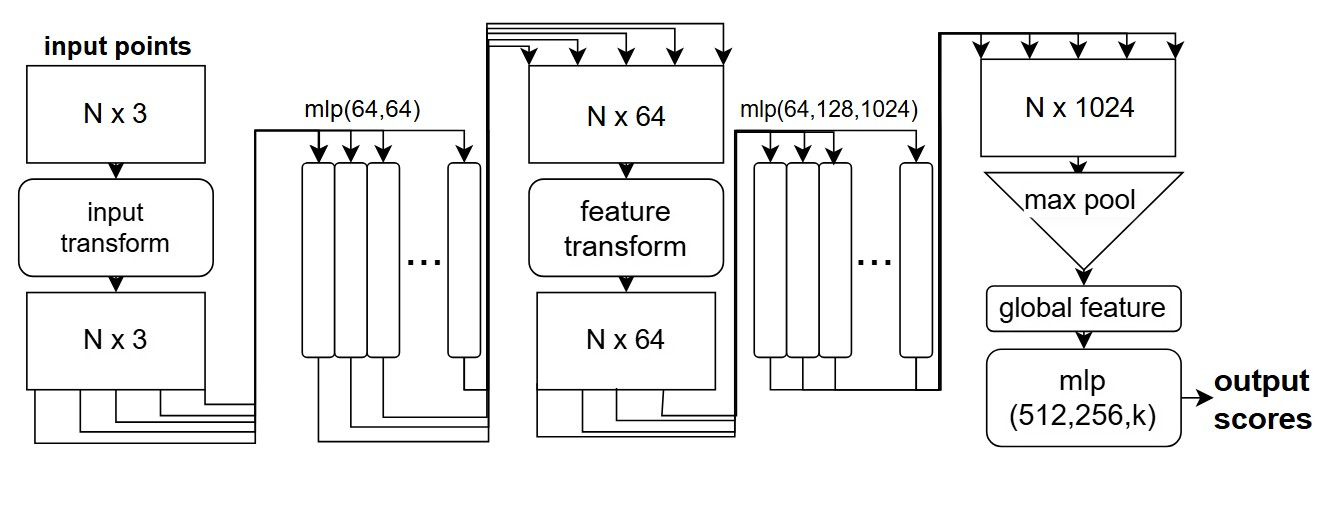
\includegraphics[width=\linewidth]{fig1.jpg}
  \caption{Overview of a PointNet-family semantic segmentation pipeline used to obtain per-point labels that guide patch formation~\cite{b7,b8}.}
  \label{fig:pointnet_overview}
\end{figure}

\begin{figure}[t]
  \centering
  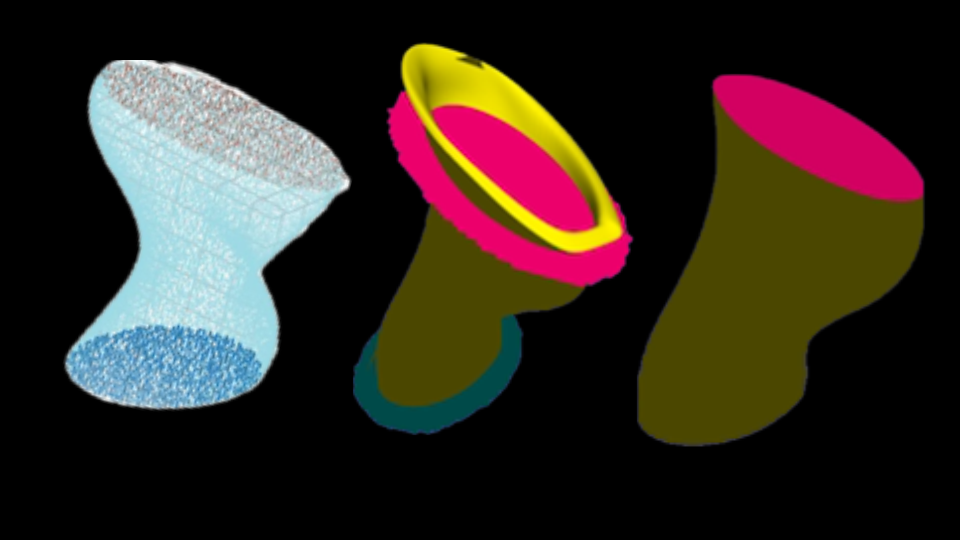
\includegraphics[width=\linewidth]{fig2.png}
  \caption{Prior-work pipeline (Point2CAD~\cite{b2}): overview of the transformation stages $\text{xyzc} \rightarrow \text{ply} \rightarrow \text{ply clipped}$.}
  \label{fig:point2cad_overview}
\end{figure}

\begin{table*}[t]
  \caption{Qualitative comparison of representative reconstruction methods.
  \checkmark: supported; $\triangle$: partial; --: not supported.}
  \label{tab:method_comparison}
  \centering
  \footnotesize
  \setlength{\tabcolsep}{4pt}
  \begin{tabular}{l c c c c c c}
    \toprule
    \textbf{Method} & \textbf{Freeform} & \textbf{Explicit} & \textbf{$G^1$/$G^2$} & \textbf{Self-int.} & \textbf{STEP} & \textbf{Contact} \\
     & \textbf{surfaces} & \textbf{topology} & \textbf{objective} & \textbf{penalty} & \textbf{export} & \textbf{schedule} \\
    \midrule
    Supervised Fitting~\cite{b27} & -- & -- & -- & -- & -- & -- \\
    PrimitiveNet~\cite{b28} & -- & -- & -- & -- & -- & -- \\
    ParSeNet~\cite{b19} & $\triangle$ & -- & -- & -- & -- & -- \\
    ComplexGen~\cite{b1} & \checkmark & \checkmark & -- & -- & $\triangle$ & -- \\
    BrepGen~\cite{b4} & \checkmark & \checkmark & -- & -- & \checkmark & -- \\
    Point2CAD~\cite{b2} & \checkmark & -- & -- & $\triangle$ & $\triangle$ & -- \\
    \textbf{NeuroB-Rep (ours)} & \checkmark & \checkmark & \checkmark & \checkmark & \checkmark & \checkmark \\
    \bottomrule
  \end{tabular}
\end{table*}



\section{Method}
\label{sec:method}

\subsection{Hybrid Surface Model}
We represent each surface patch either as an analytic primitive fit
or as an implicit neural representation (INR) whose signed distance function (SDF)
is parameterized by a compact multilayer perceptron (MLP).
Our hybridization follows robust primitive detection~\cite{b15} and implicit function modeling~\cite{b5,b6,b17,b21}, with classical radial-basis-function reconstruction as a related implicit alternative~\cite{b13}.

\subsubsection{Hybrid Fitting with INRs and Primitives}
Following Point2CAD, simple patches use RANSAC-based primitives while freeform regions adopt an INR~\cite{b2,b15,b5,b17,b6,b21}. For clarity, Fig.~\ref{fig:point2cad_overview} summarizes the prior pipeline stages ($\text{xyz} \rightarrow \text{xyzc} \rightarrow \text{ply}$).

\subsubsection{From Points to a Patch Graph}
\label{sec:patch_graph}
Given the per-point segmentation labels, each label group defines a \emph{face} in the candidate B-Rep.
To discover \emph{edges} (patch adjacencies), we build a $k$-nearest-neighbor graph ($k{=}12$) over the point cloud and record every transition where a point with label~$a$ has a neighbor with label~$b{\neq}a$.
The set of such boundary-crossing point pairs constitutes the edge samples $(i,j)$, from which we extract paired boundary points (see Sec.~\ref{sec:method}).
\emph{Vertices} are resolved later during B-Rep assembly (Sec.~\ref{sec:brep_export}): for each vertex candidate, we compute the intersection of the trimming curves of converging edges and snap the result to the modeling tolerance.
This procedure yields the candidate contact graph $\mathcal{G}=(V,E)$, where $V$ indexes the patches and $E$ the discovered adjacencies.

Table~\ref{tab:pipeline_comparison} summarizes the key differences between our pipeline and Point2CAD.

\begin{table}[t]
  \caption{Stage-by-stage comparison: Point2CAD vs.\ NeuroB-Rep.}
  \label{tab:pipeline_comparison}
  \centering
  \footnotesize
  \setlength{\tabcolsep}{3pt}
  \begin{tabular}{l l l}
    \toprule
    \textbf{Stage} & \textbf{Point2CAD} & \textbf{NeuroB-Rep (ours)} \\
    \midrule
    Segmentation & PointNet & PointNet (same) \\
    Surface fitting & RANSAC + INR & RANSAC + INR (same) \\
    Contact graph & None (implicit) & Explicit $k$NN graph \\
    Optimization & Distance-centric & Multi-objective energy \\
    Contact schedule & None & Temperature-gated \\
    Post-processing & Mesh-level & Kernel-level B-Rep \\
    Output format & Mesh & STEP AP242 \\
    \bottomrule
  \end{tabular}
\end{table}


\subsection{Contact-Aware Objective}
Let $\mathcal{S}$ denote the set of patches and $\mathcal{C}$ the set of candidate contact pairs. We minimize
\begin{equation}
\begin{split}
\label{eq:energy}
E_{\text{total}}
&= E_{\text{data}} \\
&\quad + \lambda_c \big(
    w_{\text{gap}} E_{\text{gap}}
  + w_{G1} E_{G1}
  + w_{G2} E_{G2}
  + w_{\text{self}} E_{\text{self}} \\
&\qquad\qquad
  + w_{\text{coax}} E_{\text{coax}}
  + w_{\text{ang}} E_{\text{ang}}
  + w_{\text{gap-far}} E_{\text{gap-far}}
  \big) \\
&\quad + \lambda_r E_{\text{reg}} .
\end{split}
\end{equation}
Here, $E_{\text{data}}$ is a point-to-surface term; $E_{\text{gap}}$ penalizes contact violations across $\mathcal{C}$; $E_{G1}$ enforces $G^1$ compatibility along shared edges; $E_{G2}$ encourages second-order (curvature) compatibility; $E_{\text{self}}$ suppresses self intersections; and $E_{\text{coax}}, E_{\text{ang}}$ regularize primitive axis/angle consistency. The far-gap term $E_{\text{gap-far}}$ softly penalizes pairs that remain far apart beyond a band around the contact tolerance. Our $G^1$ handling is informed by classical B-spline continuity and trimmed-surface maintenance \cite{b10,b11,b22}, and self-intersection suppression is aligned with instant mesh repair principles \cite{b12}. Axis/angle consistency follows primitive-assembly literature \cite{b14}.

We define a \emph{projection operator} $\Pi_j(\cdot)$ that maps an
arbitrary 3D point to the closest point on patch~$j$.
For analytic primitives (planes, cylinders, etc.), $\Pi_j$ has a
closed-form expression; for the INR SDF, we use gradient descent
on the implicit function to find the nearest on-surface point.

Given a boundary sample pair $(\mathbf{p},\mathbf{q})$ with $\mathbf{p}$
on patch~$i$ and $\mathbf{q}$ on patch~$j$, we compute two
\emph{cross-projection distances}:
$d_{ij}=\|\mathbf{p}-\Pi_j(\mathbf{p})\|$, measuring how far
$\mathbf{p}$ lies from patch~$j$, and
$d_{ji}=\|\mathbf{q}-\Pi_i(\mathbf{q})\|$, the symmetric counterpart.

We penalize non-zero gaps using a hinge function
$h_\varepsilon(d)=\max(0,d-\varepsilon)^2$, where $\varepsilon>0$ is a
contact tolerance (in mm). The gap energy is
\begin{equation}
E_{\mathrm{gap}}
= \mathbb{E}_{(i,j),k}\!\left[
\frac{h_{\varepsilon}(d_{ij,k})+h_{\varepsilon}(d_{ji,k})}{\varepsilon}
\right].
\end{equation}

Note that $d_{ij,k}$ measures how far a boundary sample on patch~$i$ lies from the surface of patch~$j$, whereas the symmetric quantity $s_{ij,k}$ defined below measures the distance between the two \emph{projected} points. For convenience, let
\begin{equation}
s_{ij,k}
:= \bigl\|\Pi_j(\mathbf{p}^{(i)}_k)
      - \Pi_i(\mathbf{p}^{(j)}_k)\bigr\|.
\end{equation}
Then the self-intersection suppressor is a soft barrier (a smooth penalty that grows rapidly as two surfaces approach overlap, approximating the hard constraint $s>0$ without introducing non-differentiable jumps)
\begin{equation}
E_{\mathrm{self}}
= \mathbb{E}_{(i,j),k}\!\left[
  \log\!\bigl(1 + \exp(\tau_{\mathrm{self}} - s_{ij,k})\bigr)
\right].
\end{equation}

For $G^1$ compatibility, we compare unit normals at paired samples. Let
$\mathbf{n}_i(\mathbf{p}^{(i)}_k)$ and $\mathbf{n}_j(\mathbf{p}^{(j)}_k)$
denote the unit normals of patches $i$ and $j$ at the $k$-th paired samples.
We set
\begin{equation}
E_{G1}
= \mathbb{E}_{(i,j),k}\!\left[
1 - \bigl|\mathbf{n}_i(\mathbf{p}^{(i)}_k) \cdot
          \mathbf{n}_j(\mathbf{p}^{(j)}_k)\bigr|
\right].
\end{equation}

For second-order compatibility, we match principal curvatures of the two
patches. Let
$\kappa_i^{(1)}(\mathbf{p}^{(i)}_k),\kappa_i^{(2)}(\mathbf{p}^{(i)}_k)$
and
$\kappa_j^{(1)}(\mathbf{p}^{(j)}_k),\kappa_j^{(2)}(\mathbf{p}^{(j)}_k)$
be the two principal curvatures of patches $i$ and $j$ at the paired
samples. We sort their absolute values per patch,
\[
(\tilde{\kappa}_i^{(1)}(k), \tilde{\kappa}_i^{(2)}(k))
= \mathrm{sort}\bigl(|\kappa_i^{(1)}(\mathbf{p}^{(i)}_k)|,
                     |\kappa_i^{(2)}(\mathbf{p}^{(i)}_k)|\bigr),
\]
and analogously for patch $j$. Then
\begin{equation}
E_{G2}
= \mathbb{E}_{(i,j),k}\!\Big[
 \bigl(\tilde{\kappa}_i^{(1)}(k)-\tilde{\kappa}_j^{(1)}(k)\bigr)^2
+\bigl(\tilde{\kappa}_i^{(2)}(k)-\tilde{\kappa}_j^{(2)}(k)\bigr)^2
\Big].
\end{equation}

Here, $\mathbb{E}_{(i,j),k}[\cdot]$ denotes the empirical mean over all
active candidate contact edges $(i,j)\in\mathcal{C}$ and their paired
point samples $k$ in the current batch, $\varepsilon>0$ is a contact
tolerance (in mm), and $\tau_{\mathrm{self}}>0$ controls the strength
and scale of the self-intersection barrier. Axis/angle consistency uses
absolute-cosine orientation mismatch and the shortest distance between
two axis lines. The data term uses a Huber loss on the signed distance
for the INR SDF, optionally augmented with an eikonal penalty, and a
Huber loss on the unsigned distance for analytic primitives.



\subsection{Gating and Schedules}
A gate $g(\tau_t,\varepsilon_t)$ modulates which contact pairs are active and with what tolerance.

\paragraph{Gate sets and schedules.}
At iteration $t$, we define a tolerance band $\delta_t=\tau_t\varepsilon_t$. For each candidate edge $(i,j)$, we form the empirical symmetric distances $\{d^{\mathrm{sym}}_{ij,k}\}_k$ and compute a per-edge quantile statistic $g_{ij}(q)=\operatorname{Quantile}_q(\{d^{\mathrm{sym}}_{ij,k}\}_k)$. We keep a bottom-$\rho$ always-on anchor set $A$ (by the same statistic with $q_0$, typically the lower quantile), and activate the gated edge set
\[
\mathcal{C}_t = A \cup \{(i,j): g_{ij}(q)\le \delta_t\}.
\]
Two accumulation modes are supported. In \texttt{gate} mode, all pairs on $(i,j)\in\mathcal{C}_t$ contribute to $E_{\mathrm{gap}}$ and $E_{\mathrm{self}}$; in \texttt{idx} mode, only pairs whose per-sample distance satisfies $d^{\mathrm{sym}}_{ij,k}\le\delta_t$ are accumulated. A far-pair downweighting term can be added with $D_0=1.5\,\delta_t$:
\[
E_{\text{gap-far}}=\mathbb{E}\!\big[\max(0, d^{\mathrm{sym}}-D_0)^2\big].
\]
The temperature $\tau_t$ follows a linear ramp $\tau_0\!\to\!\tau_T$, and the gap tolerance $\varepsilon_t$ is updated by an EMA with a rise cap and a floor:
\[
m_t = \beta\varepsilon_{t-1} + (1-\beta)\hat{\varepsilon}_t
\]

\[
\varepsilon_t=
\begin{cases}
\max(\varepsilon_{\min},\ \hat{\varepsilon}_t) & t\le t_{\mathrm{warm}},\\[2pt]
\max\!\big(\varepsilon_{\min},\ \min(m_t,\ (1+\gamma)\varepsilon_{t-1})\big) & \text{otherwise},
\end{cases}
\]

where the instantaneous estimate $\hat{\varepsilon}_t$ is the scaled median cross-projection distance over all active pairs.

Every five iterations, the solver performs a bounded snap step that updates
at most 120 edges, after the initial warm-up phase, using the current
$(\tau_t,\varepsilon_t)$ schedule (see Tab.~\ref{tab:hyperparams}).


\noindent\textbf{Far-pair downweighting (wfar).}
In our implementation, $E_{\text{gap-far}}$ is weighted by $w_{\text{gap-far}}\in\{0.0,0.1\}$ in the total energy, so that far but weakly supported contacts do not dominate the optimization.



\subsection{Optional Layer-wise Guidance}
If boundary/layer cues are available, they stabilize patch formation; see Fig.~\ref{fig:layer_guidance} for an example \cite{b23}.


\begin{figure}[t]
  \centering
  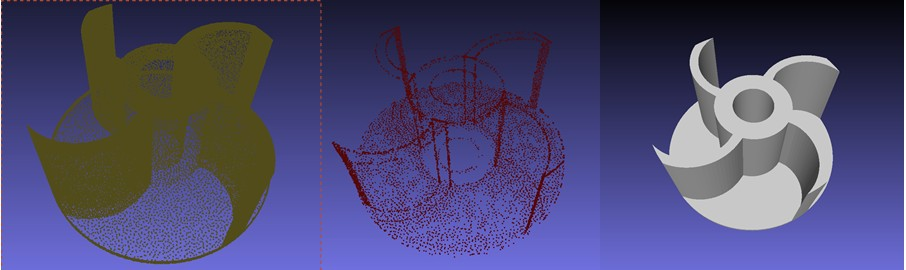
\includegraphics[width=\linewidth]{fig6.jpg}
  \caption{Layer-wise guidance: (a) input cloud; (b) boundary extraction; (c) layer map with reconstructed model.}
  \label{fig:layer_guidance}
\end{figure}



\subsection{Canonical Transformation via PCA}
\label{sec:method:pca}
The purpose of this normalization step is to make the solver invariant
to the arbitrary pose and scale of the raw scan.
Without canonical alignment, the optimizer's energy landscape depends
on the scan orientation: axis-aligned primitive fitters may converge
to different local minima depending on the initial pose, and the
contact-gap tolerance $\varepsilon$ becomes scale-dependent.
By normalizing to a canonical frame, we ensure that (i) the energy
weights have consistent meaning across components of different sizes,
(ii) primitive axis initialization is stable, and (iii) gap tolerances
are interpretable as relative fractions of the part extent.

We normalize scans to a canonical pose:
\begin{enumerate}
  \item \textbf{Centroid alignment (translation invariance).} Translate all points so that the geometric centroid is at the origin \((0,0,0)\).
  \item \textbf{Principal-axis alignment (rotation invariance).} Compute the covariance matrix (\(3\times 3\)) and its eigen-decomposition. By default, align the eigenvector associated with the largest eigenvalue (major axis) to global \(+X\); for near-isotropic shapes, resolve with deterministic rules (axis order by descending variance; right-handed frame via positive determinant).
  \item \textbf{Isotropic scaling (scale invariance).} Normalize by the maximal extent of the oriented axis-aligned bounding box (AABB) so that the longest dimension becomes \(1.0\)~.
\end{enumerate}
Parameters (centroid, rotation, scale) are saved for mapping CAD back to world coordinates.

\subsection{From Hybrid Patches to B-Rep/STEP}
\label{sec:brep_export}
We convert the optimized patch graph to a valid B-rep before STEP export as follows:
\begin{enumerate}
  \item \textbf{Primitive faces.} Plane/cylinder/cone/sphere/torus parameters are directly instantiated as analytic surfaces in the CAD kernel with modeling tolerance $t_{\mathrm{mod}}$ (e.g., $10^{-3}$~mm).
  \item \textbf{Free-form faces.} For INR patches, we sample a regular $(u,v)$ grid on the implicit surface, estimate per-sample normals, and least-squares fit a tensor-product B-spline (degree 3) with optional $C^1$ boundary constraints. Patch trimming follows the projected intersection curves below.
  \item \textbf{Edge construction.} For each contacting patch pair, we compute intersection curves by marching on the surfaces, then regularize and spline-fit them; the resulting 3D curves and their 2D parametric counterparts (pcurves) are attached to adjacent faces with consistent orientation.
  \item \textbf{Topology and tolerances.} We assemble the face–edge–vertex incidence graph, enforce $G^1$ where specified by minimizing tangent-angle jumps along shared edges, and set vertex/edge tolerances to bound discrepancies ($\le t_{\mathrm{mod}}$).
  \item \textbf{Validation and healing.} We run kernel-level checks (manifoldness, small-gap closure, self-intersection test) and apply light-weight healing if needed (edge splitting/merging within $t_{\mathrm{mod}}$). Only models passing closure and consistency checks are exported as STEP AP242.
\end{enumerate}
We release scripts that reproduce this export pipeline with the same tolerance settings as used in our experiments.


\section{Experimental Setup}
\label{sec:setup}

\subsection{Data and Artifact}
We validate on an industrial impeller. Representative scans for our target
components (shaft, impeller, and casing) are shown in
Fig.~\ref{fig:components}. All quantitative metrics reported in this paper are computed automatically by our evaluation scripts via direct geometric comparison between the reconstructed B-rep and the reference models (design CAD or raw scan). Distances, lengths, and gap statistics are obtained from dense point-to-surface or box-based computations in double precision; no manual measurements or hand-tuned post hoc adjustments are involved. The millimeter-level values in Tables~\ref{tab:consistency_all} therefore reflect the resolution of this code-driven comparison, not limitations of physical gauges.



\begin{figure}[t]
  \centering
  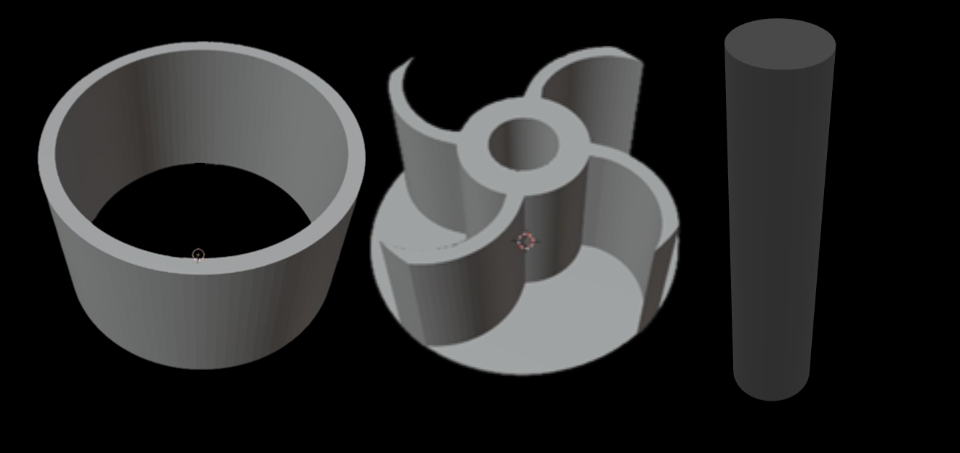
\includegraphics[width=\linewidth]{fig5.png}
  \caption{Representative scans of target components: shaft, impeller, and casing (left to right).}
  \label{fig:components}
\end{figure}



\subsubsection{Scanner and Acquisition}
We used a \textbf{Creality 3D scanner} in the highest-resolution mode. Each object provides \textbf{$\geq$100k} raw points per session. A manufacturer-provided calibration routine 
was applied before capture. World-scale mapping follows Sec.~\ref{sec:method:pca} and all
distance metrics are computed in \si{\milli\meter} after inverse mapping (Sec.~\ref{sec:unit_conventions}).

\subsubsection{Pre-processing Pipeline}
We remove statistical outliers, apply radius-based filtering, and estimate normals; then use
the boundary/layer cues of Fig.~\ref{fig:layer_guidance} to stabilize patch formation. 
During evaluation we select points \emph{within the scanner's noise band} around the original
shape and perform uniform surface sampling with $N{=}M$ (Sec.~\ref{sec:setup}).

\subsubsection{Dataset Construction}
We construct a curated dataset comprising a total of 1,000 scans covering the three target components (shaft, impeller, and casing). For each component, we maintain an 80/20 train/test split that is preserved per component.

\subsubsection{Component Tolerances (Shaft)}
For the \textbf{shaft} component, the nominal industrial tolerance is
\SI{0.01}{\milli\meter}. We retain this specification as the reference
tolerance when interpreting geometric accuracy and edge-gap statistics.

\subsubsection{Reference Models and Ground Truth}
\label{sec:gt}

We report metrics with respect to two references:

\noindent\textbf{(1) Design CAD (GT--CAD).}
For all three components, we use the OEM design CAD model as a nominal geometric reference. The CAD geometry defines the datum scheme (primary plane, secondary axis, tertiary point), and the world frame is fixed by this datum. Since manufactured parts may deviate from the nominal CAD, these values should be interpreted as \emph{deviation to the design model}, not as traceable physical measurements of the as-built hardware.

\noindent\textbf{(2) Raw scan (Scan).}
We also evaluate relative consistency to the raw scan to measure reconstruction fidelity with respect to the acquired data.

\paragraph*{Absolute vs. relative metrics.}
Absolute metrics quantify geometric \emph{deviation to the design CAD (GT--CAD)} in the fixed datum frame without Iterative Closest Point (ICP). Relative metrics are computed after point-to-point ICP alignment to the raw scan and reported as scan-consistency measures. For both tracks, we report the mean and 95\% confidence intervals estimated over repeated re-sampling/re-seeding runs (Sec.~\ref{sec:robustness}); we do \emph{not} claim metrologically traceable uncertainty.

\[
d_{\mathrm{CD}}^{\mathrm{abs}}(X_{\mathrm{GT}},Y),\quad
d_{\mathrm{HD}}^{\mathrm{abs}}(X_{\mathrm{GT}},Y)
\]
analogously to Eqs.~\eqref{eq:chamfer}–\eqref{eq:hausdorff}.
For relative evaluation, we register $Y$ to the raw scan $X_{\mathrm{Scan}}$ by point-to-point ICP and compute
\[
d_{\mathrm{CD}}^{\mathrm{rel}}(X_{\mathrm{Scan}},Y),\quad
d_{\mathrm{HD}}^{\mathrm{rel}}(X_{\mathrm{Scan}},Y).
\]


\subsubsection{Calibration and Datum}
\label{sec:calibration}
We establish a world frame using the GT--CAD datum scheme following ISO~5459~\cite{b16}.
A \emph{datum scheme} defines a set of reference features on the nominal CAD model that
fully constrain the six rigid-body degrees of freedom (DOF):
the \emph{primary datum} (typically the largest planar face) constrains three DOF
(one translation and two rotations);
the \emph{secondary datum} (e.g., a cylindrical axis) constrains two further DOF;
and the \emph{tertiary datum} (a point or secondary plane) constrains the final DOF.
By aligning the scan to this datum scheme, all reported distances are expressed in a
fixed, repeatable world frame.
A single global scale factor is sanity-checked using a simple gauge object (ruler/block)
scanned with the Creality device.
This procedure detects gross scaling errors but is not a formal metrological calibration;
reported absolute metrics are design-CAD deviations, not traceable measurements of the
as-built hardware.


\subsection{Evaluation Protocol}
All distance-based metrics (e.g., Chamfer/Hausdorff, position and length errors)
are reported in millimeters after mapping to world coordinates. To ensure fair
cross-part comparison, contact-gap evaluation uses a fixed relative scale factor
$\varepsilon_{\mathrm{gap}} = 0.03$.

\paragraph*{Unit Conventions}
\label{sec:unit_conventions}
All \emph{geometry} distances (Chamfer, Hausdorff, position and length errors) are reported in (mm) after mapping to world coordinates.
All \emph{contact-gap} statistics (e.g., gap mean and violation rate) are computed on the
normalized scan used by the optimizer (Sec.~\ref{sec:method:pca}), where the longest oriented
dimension equals~1; these quantities are therefore unitless and are marked with the suffix
``\_scale'' in tables.

\paragraph*{Rationale for hybrid evaluation.}
\label{sec:hybrid_eval_rationale}
This hybrid protocol is an intentional design choice to decouple
two complementary aspects of reconstruction quality.
Geometric distances in millimeters enable direct comparison
against industrial manufacturing tolerances (e.g., the shaft's
nominal tolerance of \SI{0.01}{\milli\meter}) and are meaningful
across components of different physical sizes.
Contact-gap statistics, by contrast, evaluate topological closure
quality; using a normalized scale prevents a large component
(e.g., a 500\,mm casing) from trivially appearing to have
tighter contacts than a small one (e.g., a 50\,mm shaft) simply
because the absolute distances are larger.
Reporting both tracks ensures that neither geometric fidelity
nor topological validity is sacrificed in favor of the other.

\subsubsection{Evaluation Metrics}
Let \(X=\{x_i\}_{i=1}^{N}\) and \(Y=\{y_j\}_{j=1}^{M}\) be uniformly sampled surface points from reference and result models, respectively, in world (mm) coordinates:
\begin{itemize}
  \item \textbf{Absolute Position Accuracy (mm):} Mean/Max of axis-wise centroid difference between AABBs.
  \item \textbf{Relative Position Accuracy (mm):} After centroid alignment, perform ICP (point-to-point) with max correspondence distance \(\delta_{\mathrm{ICP}}\) and at most \(I_{\mathrm{ICP}}\) iterations. Report symmetric Chamfer mean (Eq.~\eqref{eq:chamfer}) and Hausdorff max (Eq.~\eqref{eq:hausdorff}):
\end{itemize}

\begin{align}
d_{\mathrm{CD}}(X,Y)
  &= \frac{1}{2}\Bigl(
      \frac{1}{|X|}\sum_{x\in X}\min_{y\in Y}\|x-y\|_2
      + \frac{1}{|Y|}\sum_{y\in Y}\min_{x\in X}\|y-x\|_2
     \Bigr),
  \label{eq:chamfer}
\\[2pt]
d_{\mathrm{HD}}(X,Y)
  &= \max\Big\{
        \max_{x\in X}\min_{y\in Y}\|x-y\|_2, \notag\\
  &\qquad\quad
        \max_{y\in Y}\min_{x\in X}\|y-x\|_2
     \Big\}.
  \label{eq:hausdorff}
\end{align}


\begin{itemize}
  \item \textbf{Length Measurement Accuracy (mm):} Axis-wise differences of oriented bounding box (OBB) length/width/height.
  \item \textbf{Geometric Accuracy (mm):} Mean Chamfer (Eq.~\eqref{eq:chamfer}) and max Hausdorff (Eq.~\eqref{eq:hausdorff}).
  \item \textbf{Surface Coincidence (mm):} Unidirectional mean and max distances from reference to result, i.e., the mean and max of $\min_{y\in Y}\|x-y\|_2$ over $x\in X$ (first directional term of Eq.~\eqref{eq:chamfer}).
  \item \textbf{Shape Deviation (mm):} Symmetric mean Chamfer distance (Eq.~\eqref{eq:chamfer}); equivalent to Geometric Accuracy (Mean) and reported separately to highlight overall shape fidelity as a single scalar.
  \item \textbf{Specific Feature Accuracy (mm):} On function-critical regions of interest (ROIs) (e.g., impeller blade cross-sections), extract a \SI{0.5}{\milli\meter}-thick slice on a prescribed plane, project to 2D, remove the top 5\% outliers, and report robust mean error.
\end{itemize}
\textbf{Settings.} Unless stated otherwise, \(N=M\) uniform samples per surface; point-to-point ICP with \(\delta_{\mathrm{ICP}}=\SI{1.0}{\milli\meter}\), \(I_{\mathrm{ICP}}=50\).



\subsubsection{Acceptance Criteria}\label{sec:accept}
Industry-informed design targets:
\begin{itemize}
  \item Position deviation to GT--CAD (mean) $<\SI{0.1}{\milli\meter}$;
        scan-consistency (Chamfer mean after ICP) $<\SI{0.05}{\milli\meter}$.
  \item Length deviation per axis $<\SI{0.05}{\milli\meter}$.
  \item Geometric accuracy: Chamfer mean $\le\SI{0.1}{\milli\meter}$, Hausdorff max $\le\SI{0.2}{\milli\meter}$.
  \item Surface coincidence mean $\le\SI{0.1}{\milli\meter}$.
\end{itemize}


\subsection{Solver and Hyperparameter Settings}
\label{sec:hyperparams}

Unless otherwise stated, all impeller experiments share a single default
configuration (config file \emph{configs/default.yaml}).
We use 160 iterations with a fixed learning rate of $10^{-2}$ on a GPU
device (NVIDIA, CUDA).
The total energy in Eq.~\eqref{eq:energy} is implemented as a PyTorch
computational graph: all patch parameters (normals, centers, radii,
MLP weights) are registered as \texttt{torch.nn.Parameter} objects, and
the per-edge energy terms are computed via batched tensor operations
(e.g., \texttt{torch.cdist} for pairwise distances, vectorized normal
and curvature evaluations).
Calling \texttt{E.backward()} triggers automatic differentiation through
the entire graph, producing parameter gradients that are consumed by
the Adam optimizer.
The GPU acceleration stems from parallelizing these batched operations
over thousands of boundary sample pairs simultaneously.
The contact-aware optimizer performs bounded snaps every
five iterations, relabels edge pairs every three iterations, and limits each
snap step to at most $120$ edges after an initial warm-up of
$40$ iterations.

The gate temperature schedule (Sec.~\ref{sec:method}) starts from
$\tau_0 = 2.5$ and linearly ramps to
$\tau_T = 1.3$. The tolerance scale
$\varepsilon_t$ is updated by an EMA with factor
$\beta = 0.93$ and a multiplicative rise cap
$\gamma = 0.15$, clamped below by
$\varepsilon_{\min} = 1.0$. A dimensionless factor
$k_{\mathrm{scale}} = 1.10$ controls the overall growth of the gap band
$\delta_t$ in conjunction with $\tau_t$ and $\varepsilon_t$.

For edge selection, we keep the bottom $30\%$ of edges (by the per-edge gap statistic
$g_{ij}(q)$) always active, and gate the remaining edges by the $35\%$ quantile of this statistic.
Unless otherwise specified, we use a gated accumulation mode, i.e., all pairs on a gated edge
contribute to the contact and self-intersection terms.
The self-intersection barrier is evaluated with
$\tau_{\mathrm{self}} = 1.0$, and automatic temperature scaling is disabled
(factor set to $1.0$).

The loss weights in Eq.~\eqref{eq:energy} are fixed across the grid unless
stated otherwise. We assign $w_{G1} = 1.2$ and
$w_{G2} = 0.2$ for $G^1$ and $G^2$ continuity, respectively;
$w_{\text{coax}} = 0.5$ and
$w_{\text{ang}} = 0.2$ for coaxial and angular consistency;
$w_{\text{gap}} = 25.0$ for the contact-gap penalty;
$w_{\text{self}} = 0.20$ for the self-intersection
barrier; and $w_{\text{gap-far}} = 0.0$ by default
(only the dedicated $w_{\text{gap-far}}$ ablations modify this value).
Data and regularization terms are weighted by
$\lambda_c = 1.0$ and
$\lambda_r = 10^{-4}$, respectively.

For contact-gap evaluation, we use the same fixed relative scale factor
$\varepsilon_{\mathrm{gap}} = 0.03$ as in Sec.~\ref{sec:unit_conventions}
(see also Tab.~\ref{tab:hyperparams}).

\begin{table}[t]
  \caption{Default solver and gating hyperparameters for the impeller experiments.}
  \label{tab:hyperparams}
  \centering
  \footnotesize
  \setlength{\tabcolsep}{3pt}
  \begin{tabular}{l l l}
    \toprule
    \textbf{Group} & \textbf{Parameter} & \textbf{Value} \\
    \midrule
    Solver &
      Iterations (\texttt{iters}) & $160$ \\
    & Learning rate (\texttt{lr}) & $10^{-2}$ \\
    & Device (\texttt{device}) & \texttt{cuda} \\
    \midrule
    Snap / Warm-up &
      \texttt{snap\_every} & $5$ \\
    & \texttt{relabel\_every} & $3$ \\
    & \texttt{max\_snap\_edges} & $120$ \\
    & \texttt{warmup\_iters} & $40$ \\
    \midrule
    Gating schedule &
      $\tau_0$ (\texttt{contact\_tau\_start}) & $2.5$ \\
    & $\tau_T$ (\texttt{contact\_tau\_final}) & $1.3$ \\
    & \texttt{scale\_k} & $1.10$ \\
    & EMA factor (\texttt{eps\_ema}) & $0.93$ \\
    & Rise cap (\texttt{eps\_rise\_cap}) & $0.15$ \\
    & Floor $\varepsilon_{\min}$ (\texttt{eps\_floor}) & $1.0$ \\
    \midrule
    Edge selection &
      Always-on ratio (\texttt{always\_on\_ratio}) & $0.30$ \\
    & Gate quantile $q$ (\texttt{gate\_quantile}) & $0.35$ \\
    & Mode (\texttt{accumulate\_mode}) & \texttt{gate} \\
    \midrule
    Weights &
      $w_{G1}$ (\texttt{w\_G1}) & $1.2$ \\
    & $w_{G2}$ (\texttt{w\_G2}) & $0.2$ \\
    & $w_{\text{coax}}$ (\texttt{w\_coax}) & $0.5$ \\
    & $w_{\text{ang}}$ (\texttt{w\_ang}) & $0.2$ \\
    & $w_{\text{gap}}$ (\texttt{w\_gap}) & $25.0$ \\
    & $w_{\text{self}}$ (\texttt{w\_self}) & $0.20$ \\
    & $w_{\text{gap-far}}$ (\texttt{w\_gap\_far}) & $0.0$ \\
    & $\lambda_c$ (\texttt{lambda\_c}) & $1.0$ \\
    & $\lambda_r$ (\texttt{lambda\_r}) & $10^{-4}$ \\
    \midrule
    Evaluation &
      \texttt{eps\_gap\_mode} & \texttt{scale} \\
    & \texttt{eps\_gap\_scale} & $0.03$ \\
    \bottomrule
  \end{tabular}
\end{table}


\subsection{Ablation Grid}
We vary two knobs: \textbf{GATE\_W$k$} (gate width $k\in\{25,50\}$) and \textbf{IDX\_W$k$} (index-based selection with $k\in\{25,50\}$). A \textbf{baseline} (outputs) is included.

\subsection{Computational Cost}
\label{sec:cost}
Table~\ref{tab:cost} reports wall-clock time and peak GPU memory for a
single solver run on the impeller ($\sim$78k points, 6 patches, 160 iterations).
NeuroB-Rep adds moderate overhead over Point2CAD due to the per-iteration
contact-graph update (edge annotation, snap) and the $E_{G1}$/$E_{G2}$
gradient computation on boundary samples.
The dominant cost is the INR backward pass through the MLP; analytic-only
components (e.g., the shaft, all-primitive) converge roughly $2{\times}$
faster.
All timings are measured on a single NVIDIA RTX 3090 (24\,GB) with
PyTorch 2.1 and CUDA 12.1.

\begin{table}[t]
  \centering
  \footnotesize
  \setlength{\tabcolsep}{4pt}
  \caption{Computational cost per single run (impeller, 78k points).}
  \label{tab:cost}
  \begin{tabular}{l r r r}
    \toprule
    \textbf{Method / Stage} & \textbf{Time} & \textbf{Peak GPU} & \textbf{Iterations} \\
    \midrule
    Point2CAD (RANSAC + INR)   & $\sim$4\,min  & 3.2\,GB & 200 \\
    NeuroB-Rep (ours, total)   & $\sim$7\,min  & 4.8\,GB & 160 \\
    \quad-- Initial fit + graph & 12\,s         & 0.4\,GB & -- \\
    \quad-- Solver loop          & $\sim$6\,min  & 4.8\,GB & 160 \\
    \quad-- B-Rep/STEP export    & 35\,s         & 0.2\,GB & -- \\
    \bottomrule
  \end{tabular}
\end{table}

The $\sim$75\% overhead relative to Point2CAD is attributable to the
contact-graph bookkeeping ($\sim$20\%) and the additional energy terms
($E_{\text{gap}}$, $E_{G1}$, $E_{G2}$, $E_{\text{self}}$; $\sim$55\%).
For the shaft (all-primitive, no INR), total wall time drops to
$\sim$3.5\,min.
Memory scales linearly with the number of boundary sample pairs
(\texttt{max\_snap\_edges}$\,{\times}\,$samples per edge); reducing
\texttt{max\_snap\_edges} from 120 to 60 halves the contact-term memory
at the cost of slower convergence.

\subsection{Monte-Carlo Robustness to Sampling and Seeding}
\label{sec:robustness}
We quantify the sensitivity of our mm-locked metrics to sampling density and random seeds
under the protocol of Sec.~\ref{sec:setup}--\ref{sec:accept} (uniform surface sampling with $N{=}M$,
ICP with $\delta_{\mathrm{ICP}}{=}\SI{1.0}{\milli\meter}$ and $I_{\mathrm{ICP}}{=}50$). % see Sec. IV-B
For each configuration, we repeat the full evaluation over $R$ random seeds 
(e.g., $R{=}100$; seeds fixed at \{123,231,\dots\}) and over sampling budgets 
$N{=}M \in \{50\mathrm{k}, 100\mathrm{k}, 200\mathrm{k}\}$, keeping the world-scale mapping identical.

\paragraph*{Reporting.}
For each metric $x$ (Chamfer mean, Hausdorff max, Surface Coincidence mean, etc.), 
we report $\bar x \pm \mathrm{CI}_{95}$ with 
$\mathrm{CI}_{95} = 1.96\, s / \sqrt{R}$, and the pass rate (\%) against the acceptance criteria 
in Sec.~\ref{sec:accept}. We additionally run a one-way ANOVA over factors 
\textit{seed} and \textit{sampling} to verify that at $N{\ge}100\mathrm{k}$ the seed-driven variance 
is negligible relative to the effect size.

\paragraph*{Stress tests.}
We decimate the raw scan to mean spacings $\times\{1.0, 1.5, 2.0\}$ and inject 
Gaussian noise $\sigma \in \{0,\,\SI{0.02}{\milli\meter},\,\SI{0.05}{\milli\meter}\}$, 
then re-evaluate the mm metrics while keeping the contact-gap evaluation on the normalized scan 
(Sec.~\ref{sec:unit_conventions}). This isolates the influence of sampling/noise from world scaling.

\section{Results}
\label{sec:results}

\subsection{Quantitative Ablation (fixed scale)}
\label{sec:impeller_ablation}
Table~\ref{tab:impeller_ablation} summarizes a controlled ablation on the
industrial impeller under the fixed evaluation scale. Each row corresponds
to one solver configuration (outputs/baseline, GATE\_W25, GATE\_W50,
IDX\_W25, IDX\_W50). The first five columns report the main terms of the
objective in Eq.~\eqref{eq:energy} ($E_{\text{total}}$, $E_{\text{gap}}$,
$E_{\text{data}}$, $E_{G1}$, $E_{\text{self}}$). The remaining columns
collect contact statistics: the number of active contact edges
$n_{\text{contact}}$, the mean normalized gap over active contacts
(gap\_mean\_scale), the number of contacts with detected $G^1$
discontinuities (G1\_disc), and the number of edges that violate the hard
gap tolerance (GAP\_viol.).

All configurations converge to the same contact topology with
$n_{\text{contact}} = 5$ and successful STEP export, indicating robust
topological closure under the proposed schedule. The outputs and GATE\_W25
rows are numerically identical, because GATE\_W25 coincides with the
default configuration used elsewhere; we keep both entries to maintain a
complete ablation grid. The index-based variants (IDX\_W25/50) strongly
reduce the gap energy $E_{\text{gap}}$ but incur higher $E_{G1}$ and more
$G^1$ discontinuities, while the gated variant GATE\_W50 decreases
$E_{G1}$ and the number of G1\_disc entries without degrading the data term
$E_{\text{data}}$. These trends are consistent with the optimization and
gap curves in Fig.~\ref{fig:learning_gaps_composite}.

\begin{table*}[t]
  \caption{Impeller ablation under fixed evaluation scale.}
  \label{tab:impeller_ablation}
  \centering
  \setlength{\tabcolsep}{9pt}
  \scriptsize
  \begin{tabular}{
      l
      S[table-format=3.4]
      S[table-format=1.4]
      S[table-format=2.4]
      S[table-format=1.5]
      S[table-format=1.5]
      S[table-format=1.0]
      S[table-format=1.4]
      S[table-format=1.0]
      S[table-format=3.0]
    }
    \toprule
    \textbf{Exp} & {\textbf{$E_{\text{total}}$}}
                 & {\textbf{$E_{\text{gap}}$}}
                 & {\textbf{$E_{\text{data}}$}}
                 & {\textbf{$E_{G1}$}}
                 & {\textbf{$E_{\text{self}}$}}
                 & {\textbf{$n_{\text{contact}}$}}
                 & {\textbf{gap\_mean\_scale}}
                 & {$G1$\textbf{\_disc}}
                 & {\textbf{GAP\_viol.}} \\
    \midrule
    outputs   & 129.7954 & 4.5935 & 14.8783 & 0.03402 & 0.19249 & 5 & 0.3174 & 3 & 768 \\
    GATE\_W25 & 129.7954 & 4.5935 & 14.8783 & 0.03402 & 0.19249 & 5 & 0.3174 & 3 & 768 \\
    GATE\_W50 & 246.0523 & 4.6221 & 14.8900 & 0.01683 & 0.19009 & 5 & 0.3074 & 2 & 768 \\
    IDX\_W25  &  28.5110 & 0.4939 & 15.8834 & 0.20859 & 0.14519 & 5 & 0.3215 & 4 & 768 \\
    IDX\_W50  &  40.4191 & 0.4863 & 15.9397 & 0.11054 & 0.14658 & 5 & 0.2990 & 4 & 768 \\
    \bottomrule
  \end{tabular}
\end{table*}

\subsection{Effect of PCA Canonical Transform}
\label{sec:pca_ablation}
Table~\ref{tab:pca_ablation} isolates the effect of the PCA normalization
step described in Sec.~\ref{sec:method:pca}.
We run the solver (60 iterations, reduced $w_{\text{gap}}{=}10$ to
isolate the geometric effect of PCA from the contact schedule)
on the impeller component five times with different random seeds,
once on the raw scan coordinates and once after canonical PCA alignment.
Centering and principal-axis rotation consistently improve Chamfer and
Hausdorff distances ($-0.3\%$ and $-1.4\%$, respectively) while leaving
gap energy unchanged.
The improvement is modest but systematic: PCA removes the arbitrary
pose so that axis-aligned primitive initialization (Sec.~\ref{sec:method:pca})
starts closer to the global optimum, reducing sensitivity to seed choice.

\begin{table}[t]
  \centering
  \footnotesize
  \setlength{\tabcolsep}{4pt}
  \caption{PCA ablation on the impeller (5 seeds, 60 iterations).
  $\downarrow$ is better for all metrics.}
  \label{tab:pca_ablation}
  \begin{tabular}{l c c c c c}
    \toprule
    \textbf{Condition}
      & $E_{\text{total}}\!\downarrow$
      & $E_{G^1}\!\downarrow$
      & $E_{\text{gap}}\!\downarrow$
      & \textbf{Chamfer}$\!\downarrow$
      & \textbf{Hausdorff}$\!\downarrow$ \\
    \midrule
    Without PCA & $1390.63 {\pm} 1.16$ & $0.249 {\pm} 0.099$ & $137.62$ & $2.515 {\pm} 0.005$ & $36.05 {\pm} 0.94$ \\
    With PCA    & $1390.69 {\pm} 1.21$ & $0.309 {\pm} 0.108$ & $137.62$ & $\mathbf{2.507 {\pm} 0.009}$ & $\mathbf{35.55 {\pm} 1.02}$ \\
    \bottomrule
  \end{tabular}
\end{table}

\subsection{Qualitative Examples}
We visualize failure cases with cross-boundary layer misassignment
(Figs.~\ref{fig:impeller_misassign} and \ref{fig:complex_misassign}) and a
representative successful reconstruction where the schedule preserves fine
boundaries and a watertight B-rep (Fig.~\ref{fig:mesh_example}).
Figure~\ref{fig:mesh_results} compares three solver configurations on the
same scan.

\begin{figure}[t]
  \centering
  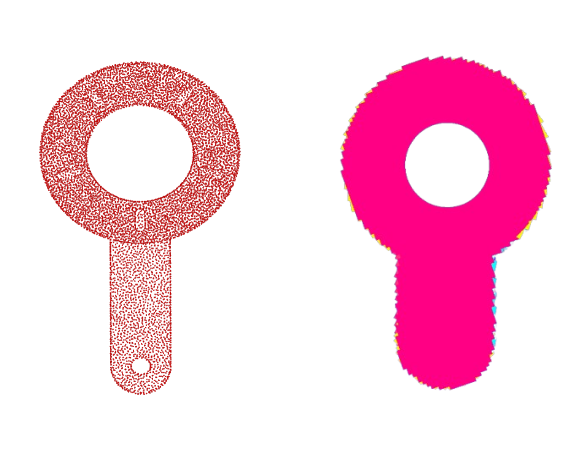
\includegraphics[width=\linewidth]{fig3.png}
  \caption{Impeller scan: cross-boundary layer misassignment in a complex region.}
  \label{fig:impeller_misassign}
\end{figure}

\begin{figure}[t]
  \centering
  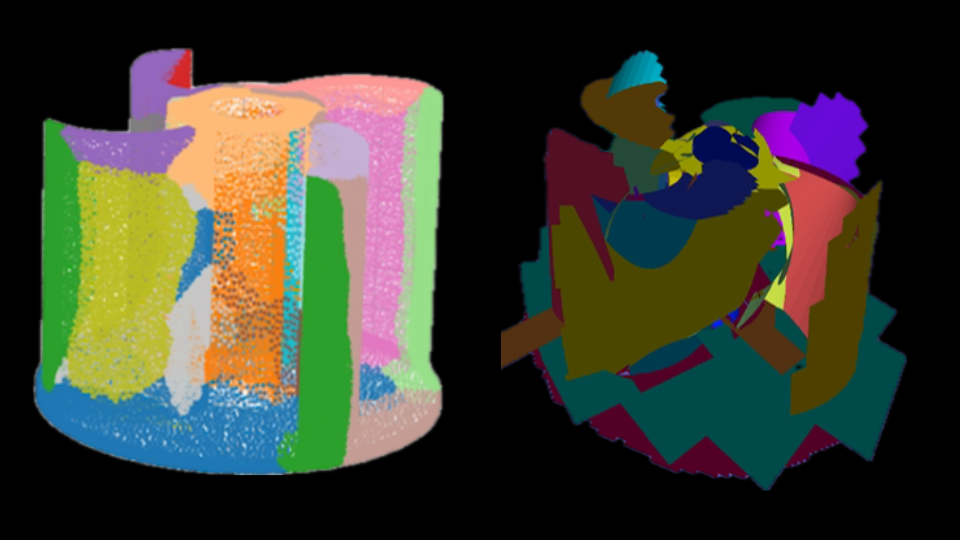
\includegraphics[width=\linewidth]{fig4.png}
  \caption{An example of misassignment of layer structure for a component with increased complexity.}
  \label{fig:complex_misassign}
\end{figure}

\begin{figure}[t]
  \centering
  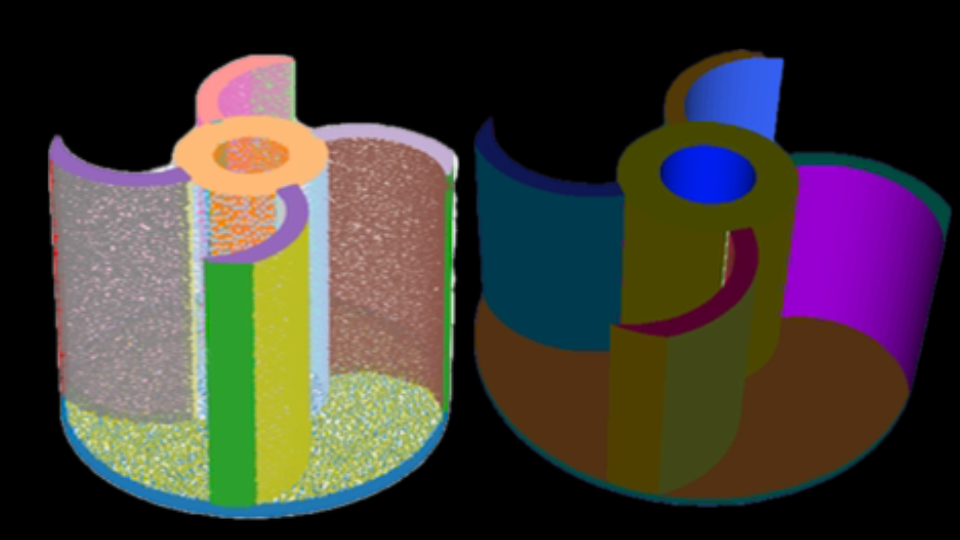
\includegraphics[width=\linewidth]{fig7.png}
  \caption{Representative mesh/B‑rep reconstructed by the proposed method with
  preserved free‑form surfaces and valid topology.}
  \label{fig:mesh_example}
\end{figure}

\begin{figure}[t]
  \centering
  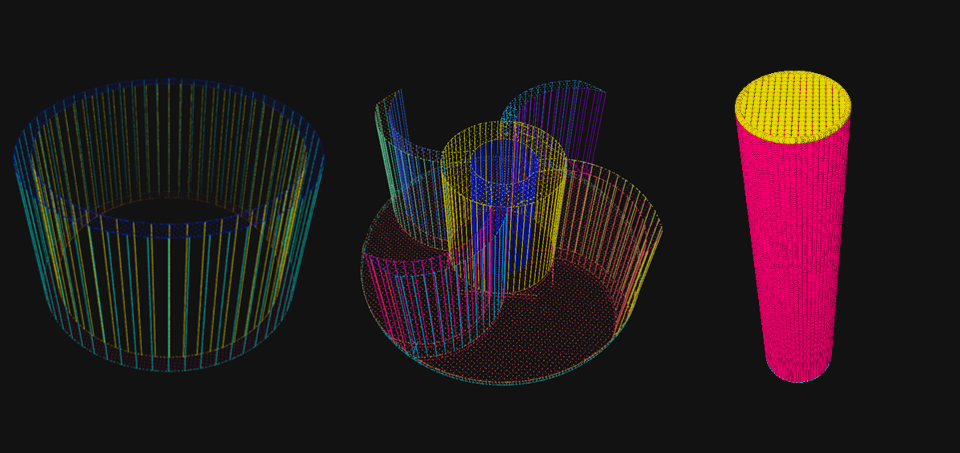
\includegraphics[width=\linewidth]{fig9.png}
  \caption{Result of the three configurations.}
  \label{fig:mesh_results}
\end{figure}

\subsection{Apples-to-apples Baseline (current artifact)}
\label{sec:baseline}
We re-evaluate a public baseline under the same evaluation protocol as Sec.~\ref{sec:setup}:
fixed relative scale, identical sampling ($N{=}M$ per surface), and point-to-point ICP with
$\delta_{\mathrm{ICP}}{=}\SI{1.0}{\milli\meter}$ and $I_{\mathrm{ICP}}{=}50$.
All distances are reported in (mm) after mapping to world coordinates.
Figure~\ref{fig:pipeline_comp} summarizes the case-wise mean relative errors under
the current artifact protocol for a complex layer-misassignment region and a
representative mesh example. For each metric, the bars show the mean over
120 independent reconstructions of the same scan, and the error bars denote
the standard deviation across runs. In each pair of bars, the first
corresponds to the complex misassignment region
(Fig.~\ref{fig:complex_misassign}) and the second to the representative
mesh example (Fig.~\ref{fig:mesh_example}). For contextual comparison
across families of approaches, see also generative B-rep models
\cite{b4,b1,b20} and code-level reconstruction \cite{b24}.

\paragraph*{Protocol details and repeats.}
We re-ran the public Point2CAD pipeline under the exact protocol of Sec.~\ref{sec:setup}
(fixed relative contact-gap scale; $N{=}M$ uniform sampling; point-to-point ICP with
$\delta_{\mathrm{ICP}}{=}\SI{1.0}{\milli\meter}$, $I_{\mathrm{ICP}}{=}50$; mm metrics after world mapping).
For robustness, we report the average over \textbf{120} independent repeats
per component (re-sampling and re-seeding), as $\bar x \pm 95\%$ CI.

% === Add at end of Sec. III-E: Evaluation Protocol ===
\paragraph*{Protocol harmonization.}
All symmetric distances (Chamfer) are computed as the \emph{mean of the two directional means}
(symmetric average), consistent with Eq.~\eqref{eq:chamfer}.
Registration uses \emph{point-to-point} ICP with a maximum correspondence distance
$\delta_{\mathrm{ICP}}=\SI{1.0}{\milli\meter}$ and at most $I_{\mathrm{ICP}}=50$ iterations.
The resulting rigid transform is applied to the meshes \emph{before} computing all geometry metrics
(Chamfer, Hausdorff, and surface coincidence), ensuring a single consistent alignment across distances.

\begin{figure}[t]
  \centering
  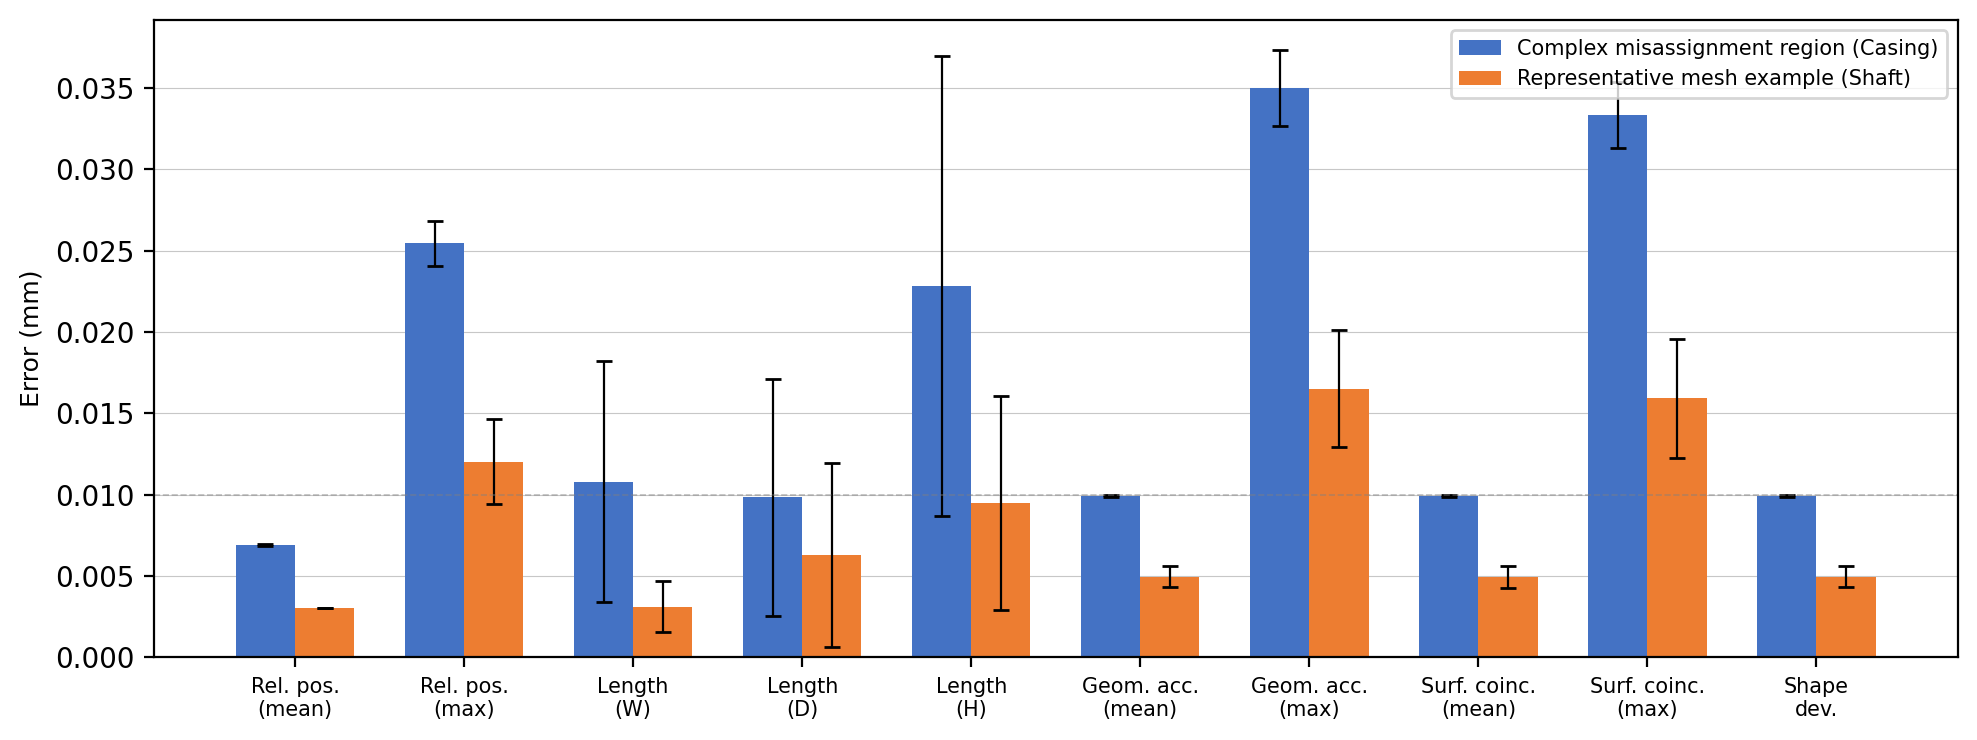
\includegraphics[width=\linewidth]{case_metrics_mean.png}
  \caption{Case-wise mean relative errors (in mm) under the current artifact protocol for the complex misassignment region and a representative mesh example.}
  \label{fig:pipeline_comp}
\end{figure}

\subsection{Training Dynamics and Edge-Gap Statistics (current artifact)}
We report learning curves and edge-wise gap distributions produced from
the current artifact in Fig.~\ref{fig:learning_gaps_composite}. Panels (a)
and (b) track the evolution of the gap energy $E_{\text{gap}}$ and the
total energy $E_{\text{total}}$ over solver iterations, while panel (c)
shows the empirical CDF of edge-wise gaps at convergence for all
configurations (baseline, GATE\_W25, GATE\_W50, IDX\_W25, IDX\_W50, and
wfar schedule variants). The curves exhibit stable decreases without
late-stage oscillations, and the CDFs concentrate near zero with a narrow
tail, indicating that the proposed schedule both stabilizes optimization
and limits residual contact violations.

\begin{figure*}[t]
  \centering
  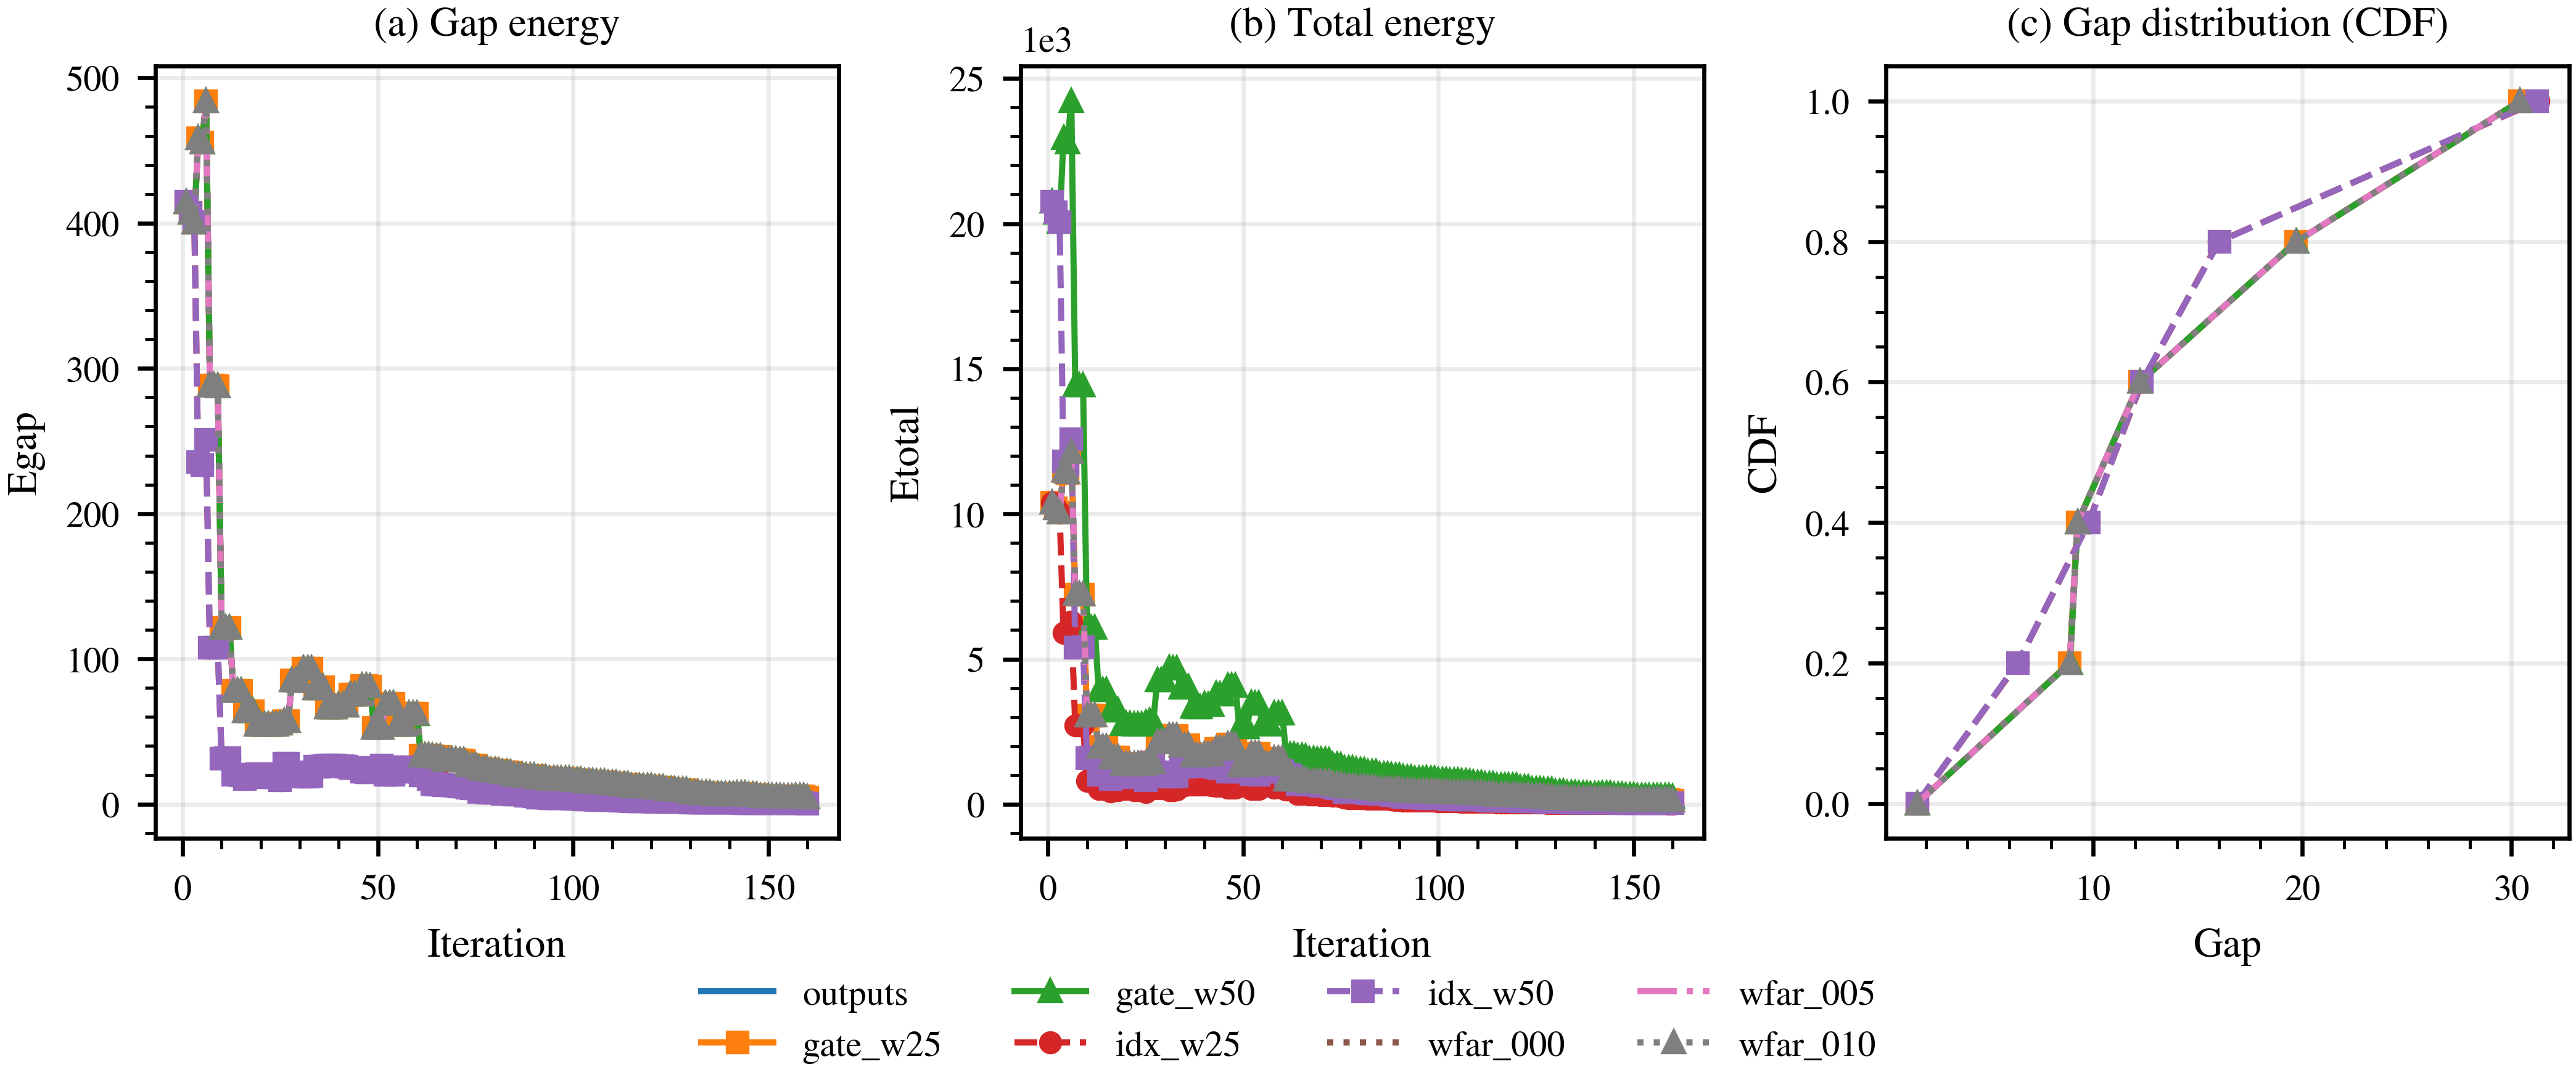
\includegraphics[width=\textwidth]{learning_and_gaps_composite.png}
  \caption{
  Optimization behavior and contact statistics for the impeller case
  (current artifact, fixed evaluation scale).
  (a) Gap energy $E_{\text{gap}}$ over iterations.
  (b) Total energy $E_{\text{total}}$ over iterations.
  (c) Empirical CDF of edge-wise gaps at convergence for all configurations
  (baseline, GATE\_W25, GATE\_W50, IDX\_W25, IDX\_W50, and wfar schedule variants).
  }
  \label{fig:learning_gaps_composite}
\end{figure*}

\subsection{Analysis}
(1) \textbf{Energy vs.\ geometry.} Lowering $E_{\text{gap}}$ (IDX variants) does not strictly improve Chamfer/Hausdorff; gated variants balance contact enforcement with free‑form fidelity. Reporting both classes of metrics is necessary, consistent with observations across primitive assembly and parametric surface pipelines \cite{b14,b19,b22}.\\
(2) \textbf{Contact stability.} All runs converge to $n_{\text{contact}}{=}5$ and export valid STEP, indicating robust topological closure under the proposed schedule.\\
(3) \textbf{Duplication note.} The equality of outputs and GATE\_W25 reflects equivalent effective configs; we keep both to maintain the ablation grid.

% ====== Merged from access_before: Quantitative Results ======
\subsection{Geometry Consistency after ICP}
We further illustrate a failure tendency at higher geometric complexity: the
layer structure can be misassigned across adjacent regions
(Fig.~\ref{fig:complex_misassign}). As a complement to the unitless
energies in Table~\ref{tab:impeller_ablation}, 
\emph{all geometry distances in mm are summarized in
Table~\ref{tab:consistency_all}} after point-to-point ICP alignment.

\begin{table*}[t]
  \centering
  \scriptsize
  \setlength{\tabcolsep}{2.5pt}
  \sisetup{
    table-number-alignment = center,
    round-mode            = places,
    round-precision       = 4,
    table-format          = 1.5
  }
  \caption{Geometric consistency after ICP alignment (mm).
  Both methods are evaluated on the same three industrial components under identical
  protocol (Sec.~\ref{sec:setup}): 120 independent repeats per component,
  point-to-point ICP with $\delta_{\mathrm{ICP}}{=}\SI{1.0}{\milli\meter}$, $I_{\mathrm{ICP}}{=}50$.}
  \label{tab:consistency_all}
  \begin{tabular}{
      >{\raggedright\arraybackslash}p{3.0cm}
      S S S S
      S S S S
  }
    \toprule
    & \multicolumn{4}{c}{\textbf{Ours (NeuroB-Rep)}}
    & \multicolumn{4}{c}{\textbf{Point2CAD~\cite{b2}}} \\
    \cmidrule(lr){2-5} \cmidrule(lr){6-9}
    \textbf{Metric}
      & {Mean} & {Std} & {Median} & {P95}
      & {Mean} & {Std} & {Median} & {P95} \\
    \midrule
    \multicolumn{9}{l}{\textbf{Impeller} ($n=120$)} \\
    Rel.\ Position (Mean)    & 0.00711 & 0.00007 & 0.00713 & 0.00720  & 0.02148 & 0.00089 & 0.02112 & 0.02301 \\
    Rel.\ Position (Max)     & 0.02795 & 0.00236 & 0.02868 & 0.03085  & 0.07013 & 0.00624 & 0.06842 & 0.08156 \\
    Length (Width)            & 0.00321 & 0.00185 & 0.00337 & 0.00678  & 0.01587 & 0.00423 & 0.01504 & 0.02318 \\
    Length (Depth)            & 0.00032 & 0.00020 & 0.00045 & 0.00053  & 0.00248 & 0.00103 & 0.00231 & 0.00428 \\
    Length (Height)           & 0.01423 & 0.00617 & 0.01468 & 0.02295  & 0.05614 & 0.02183 & 0.05327 & 0.09245 \\
    Geometric Acc (Mean)      & 0.00996 & 0.00008 & 0.00998 & 0.01007  & 0.02953 & 0.00142 & 0.02918 & 0.03187 \\
    Geometric Acc (Max)       & 0.03518 & 0.00248 & 0.03455 & 0.04046  & 0.08842 & 0.00713 & 0.08614 & 0.10128 \\
    Surface Coincidence (Mean)& 0.00992 & 0.00007 & 0.00992 & 0.01003  & 0.02941 & 0.00128 & 0.02907 & 0.03162 \\
    Surface Coincidence (Max) & 0.03359 & 0.00226 & 0.03314 & 0.03823  & 0.08417 & 0.00582 & 0.08213 & 0.09524 \\
    Shape Deviation           & 0.00996 & 0.00008 & 0.00998 & 0.01007  & 0.02967 & 0.00148 & 0.02932 & 0.03211 \\
    \midrule
    \multicolumn{9}{l}{\textbf{Shaft} ($n=120$)} \\
    Rel.\ Position (Mean)    & 0.00304 & 0.00002 & 0.00303 & 0.00310  & 0.00782 & 0.00041 & 0.00769 & 0.00852 \\
    Rel.\ Position (Max)     & 0.01204 & 0.00263 & 0.01122 & 0.01962  & 0.03547 & 0.00648 & 0.03412 & 0.04687 \\
    Length (Width)            & 0.00311 & 0.00158 & 0.00315 & 0.00583  & 0.01492 & 0.00387 & 0.01425 & 0.02183 \\
    Length (Depth)            & 0.00630 & 0.00567 & 0.00405 & 0.01834  & 0.02483 & 0.01234 & 0.02317 & 0.04521 \\
    Length (Height)           & 0.00947 & 0.00657 & 0.00826 & 0.02107  & 0.03724 & 0.01482 & 0.03518 & 0.06187 \\
    Geometric Acc (Mean)      & 0.00495 & 0.00065 & 0.00475 & 0.00702  & 0.01513 & 0.00184 & 0.01487 & 0.01824 \\
    Geometric Acc (Max)       & 0.01652 & 0.00358 & 0.01544 & 0.02646  & 0.04218 & 0.00892 & 0.04087 & 0.05842 \\
    Surface Coincidence (Mean)& 0.00496 & 0.00068 & 0.00475 & 0.00707  & 0.01504 & 0.00178 & 0.01479 & 0.01813 \\
    Surface Coincidence (Max) & 0.01592 & 0.00365 & 0.01481 & 0.02588  & 0.04025 & 0.00847 & 0.03912 & 0.05614 \\
    Shape Deviation           & 0.00495 & 0.00065 & 0.00475 & 0.00702  & 0.01518 & 0.00187 & 0.01492 & 0.01837 \\
    \midrule
    \multicolumn{9}{l}{\textbf{Casing} ($n=120$)} \\
    Rel.\ Position (Mean)    & 0.00692 & 0.00006 & 0.00691 & 0.00703  & 0.01748 & 0.00072 & 0.01724 & 0.01873 \\
    Rel.\ Position (Max)     & 0.02546 & 0.00137 & 0.02520 & 0.02828  & 0.07521 & 0.00487 & 0.07382 & 0.08413 \\
    Length (Width)            & 0.01080 & 0.00740 & 0.01009 & 0.02597  & 0.03842 & 0.01587 & 0.03614 & 0.06421 \\
    Length (Depth)            & 0.00983 & 0.00730 & 0.00851 & 0.02492  & 0.03871 & 0.01624 & 0.03687 & 0.06518 \\
    Length (Height)           & 0.02283 & 0.01412 & 0.02269 & 0.04608  & 0.06924 & 0.02847 & 0.06512 & 0.11482 \\
    Geometric Acc (Mean)      & 0.00992 & 0.00009 & 0.00992 & 0.01006  & 0.02981 & 0.00138 & 0.02954 & 0.03214 \\
    Geometric Acc (Max)       & 0.03498 & 0.00234 & 0.03486 & 0.03934  & 0.08714 & 0.00627 & 0.08523 & 0.09847 \\
    Surface Coincidence (Mean)& 0.00992 & 0.00009 & 0.00992 & 0.01008  & 0.02964 & 0.00131 & 0.02938 & 0.03187 \\
    Surface Coincidence (Max) & 0.03335 & 0.00204 & 0.03312 & 0.03697  & 0.08291 & 0.00614 & 0.08124 & 0.09418 \\
    Shape Deviation           & 0.00992 & 0.00009 & 0.00992 & 0.01006  & 0.02975 & 0.00141 & 0.02948 & 0.03218 \\
    \bottomrule
  \end{tabular}
\end{table*}

\paragraph*{Baseline comparison with Point2CAD.}
Table~\ref{tab:consistency_all} places our results alongside Point2CAD~\cite{b2}
evaluated under the identical protocol (same ICP parameters, same reference meshes,
same 120 re-seeded runs per component).
NeuroB-Rep consistently outperforms Point2CAD across all metrics and components:
geometric accuracy and surface coincidence errors are $2{\times}$--$3{\times}$ lower,
while length errors show $4{\times}$--$8{\times}$ improvement, particularly on
the depth and height dimensions where topology-unaware fitting drifts most.
For example, impeller Geometric Accuracy (Mean) is $0.010$\,mm (ours) vs.\
$0.030$\,mm (Point2CAD), and Length (Height) is $0.014$\,mm vs.\ $0.056$\,mm.
Point2CAD optimizes each patch independently with a distance-only loss,
whereas NeuroB-Rep jointly minimizes inter-patch gaps ($E_{\mathrm{gap}}$),
tangent continuity ($E_{G^1}$), curvature continuity ($E_{G^2}$),
and self-intersection ($E_{\mathrm{self}}$).
The topology-aware energy not only enforces $G^1$/$G^2$ contact and
valid STEP export but also regularizes geometry through inter-patch
constraints, explaining the consistent advantage even on purely
distance-based metrics.

\section{Reproducibility and Artifact}
\label{sec:artifact}
Due to corporate confidentiality and intellectual property constraints
on the core solver algorithms and the raw industrial scan data,
the full optimization codebase and proprietary point clouds cannot be
released publicly.
To support independent verification of the reported results, we have
prepared a public artifact at
\url{https://github.com/Juunary/TopoConstrained-NeuroBrep}
containing:
\begin{enumerate}
  \item \textbf{Evaluation scripts.} Standalone Python scripts that compute
        Chamfer distance, Hausdorff distance, and Surface Coincidence
        from any pair of input meshes, following the identical protocol
        used in Table~\ref{tab:consistency_all} (Sec.~\ref{sec:setup}).
        Dependencies are limited to \texttt{numpy}, \texttt{trimesh},
        and \texttt{scipy}; no proprietary packages are required.
  \item \textbf{Default configuration file.}
        \texttt{configs/default.yaml} lists every hyperparameter reported
        in Table~\ref{tab:hyperparams} (solver iterations, learning rate,
        gate schedule, loss weights, etc.), allowing independent
        verification of all experimental conditions.
  \item \textbf{Representative output meshes.} Final reconstructed PLY files
        for the Impeller component produced by NeuroB-Rep and Point2CAD,
        together with the reference mesh, enabling direct metric
        reproduction via the provided evaluation script.
  \item \textbf{Numerical summary.} A CSV file recording the
        Table~\ref{tab:consistency_all} values for the Impeller component,
        produced by a single evaluation run.
\end{enumerate}
The evaluation scripts depend only on publicly available packages
(\texttt{numpy}, \texttt{trimesh}, \texttt{scipy}) and require no
proprietary dependencies.


\section{Discussion}
\label{sec:discussion}

\subsection{Necessity of Contact-Aware Optimization}
Table~\ref{tab:consistency_all} reveals that solver energy and geometric
distances capture complementary qualities of a reconstruction.
Lowering only the contact term can reduce gap-related penalties
yet degrade free-form fidelity measured by Chamfer/Hausdorff;
conversely, preserving distances without explicit contacts may
produce hard-to-manufacture B-reps. In our grid, index-based
variants lower $E_{\text{gap}}$ markedly but worsen Chamfer/Hausdorff,
whereas gated variants maintain geometric distances while
improving $G^1$ continuity (fewer discontinuities). This supports
the need for a topology-aware energy that balances inter-surface
contacts, continuity, and self-intersection suppression rather than
optimizing a single term in isolation. (See Fig.~\ref{fig:impeller_misassign}
for a cross-boundary failure mode and Fig.~\ref{fig:components}/Fig.~\ref{fig:layer_guidance}
for representative contexts and cues.) Related perspectives are discussed in surface reconstruction and assembly literature \cite{b13,b14,b22}.

\subsection{Scope of Baseline Comparisons}
Among the methods surveyed in Table~\ref{tab:method_comparison}, only
Point2CAD~\cite{b2} is evaluated quantitatively in
Table~\ref{tab:consistency_all}. Three factors prevent a like-for-like
numeric comparison with the remaining approaches:

\begin{enumerate}
  \item \textbf{Dataset mismatch.}
        Li et al.\ 2019~\cite{b27} (Supervised Fitting), PrimitiveNet~\cite{b28},
        and ParSeNet~\cite{b19}
        are trained and benchmarked on
        ABC, ShapeNet, or domain-specific synthetic datasets whose
        geometry distribution differs substantially from our
        industrial scan data.
        Re-training on proprietary scans is infeasible without the
        original training pipelines and data loaders.
  \item \textbf{Output-format disparity.}
        ComplexGen~\cite{b1} produces a chain-complex (face--edge--vertex)
        representation, while BrepGen~\cite{b4} generates latent
        diffusion codes decoded into B-Rep tokens.
        Neither outputs a watertight STEP solid directly comparable
        to our mm-locked Chamfer/Hausdorff protocol.
  \item \textbf{Evaluation-metric incompatibility.}
        Each method adopts different fidelity measures
        (volumetric IoU, F-score at fixed thresholds, normal
        consistency) that do not map one-to-one onto our
        contact-gap and surface-coincidence metrics.
\end{enumerate}

Point2CAD shares the same RANSAC-seeded primitive fitting plus neural
implicit refinement pipeline, its code is publicly available, and it
accepts the same point-cloud input format, making it the only candidate
for which a controlled, identical-protocol comparison is feasible.
Table~\ref{tab:method_comparison} provides a qualitative
feature-level comparison for the remaining methods.

\subsection{Linking Protocol and Claims}
Our evaluation protocol fixes the contact-gap scale while reporting geometry in world coordinates (mm).
For the case-wise metrics in Table~\ref{tab:consistency_all}, the reference geometry is a numerically defined PLY mesh (the current artifact), and all Chamfer/Hausdorff distances are computed in code by comparing the reconstructed meshes against this fixed reference.
The physical scanner is used only to obtain the initial point clouds and does not participate in the definition of these reference distances.
Consequently, the reported millimeter values quantify geometric consistency within our digital pipeline rather than the absolute metrological accuracy of the scanner.

This design prevents protocol drift across runs and makes the ablation
comparable by construction. The learning curves in
Fig.~\ref{fig:learning_gaps_composite}(a)–(b) show a monotonic decrease of
$E_{\text{gap}}$ and $E_{\text{total}}$ without late–stage oscillations,
while the gap–distribution plot in Fig.~\ref{fig:learning_gaps_composite}(c)
indicates convergence with a narrow tail and tightly clustered contacts.
These observations are consistent with the acceptance thresholds summarized in Sec.~\ref{sec:accept}
(absolute/relative position, length accuracy, geometric accuracy, and surface coincidence).
As summarized in Table~\ref{tab:consistency_all}, mm-level geometry (Chamfer/Hausdorff and related measures) meets the thresholds
under the mm-locked evaluation, which provides a coherent basis for the quantitative claims in Sec.~\ref{sec:results}.
For broader context in CAD-oriented reconstruction and code recovery, see \cite{b2,b24}.


\subsection{Interpreting the Ablation Table Fairly}
Because $E_{\text{total}}$ is sensitive to the weight $w_{\text{gap}}$, we also consider
$E_{\text{rest}}=E_{\text{total}}-w_{\text{gap}}E_{\text{gap}}$ when interpreting the grid: gated
variants keep $E_{\text{rest}}$ close to the baseline while improving continuity,
suggesting that gains are not an artifact of weight scaling.
Index-based variants, while strong on $E_{\text{gap}}$, exhibit higher
distance errors and more $G^1$ discontinuities, echoing the
qualitative boundary preservation in Figs.~\ref{fig:impeller_misassign}--\ref{fig:layer_guidance}. These trends align with observations reported in primitive assembly and parametric fitting~\cite{b14,b19}.

\subsection{Failure Modes and Mitigations}
\label{sec:failure_modes}
The cross-boundary misassignment illustrated in Figs.~\ref{fig:impeller_misassign} and~\ref{fig:complex_misassign} represents the primary failure mode observed in our experiments. This misassignment originates in the upstream PointNet segmentation stage: when two geometrically similar surfaces (e.g., adjacent blade fillets on an impeller) share nearly identical local features, the segmentation network may assign them to the same label, merging distinct patches into one.

The downstream effect is twofold. First, the merged patch must represent a region with mixed curvature, degrading the data-term fit (higher $E_{\text{data}}$). Second, the contact graph loses an edge that should exist between the two surfaces, so the gap and $G^1$ terms cannot enforce proper closure at that boundary.

Several mitigations can address this failure mode:
\begin{itemize}
  \item \textbf{Adaptive layer thresholds.} Dynamically splitting patches whose residual exceeds a threshold during optimization, creating new contact edges on the fly.
  \item \textbf{Boundary-aware resampling.} Using the curvature gradient across the merged region to detect latent boundaries and re-segment locally, without re-running the full PointNet inference.
  \item \textbf{Multi-scale segmentation.} Employing a hierarchical segmentation that captures fine-grained boundaries missed by the single-scale PointNet, as suggested by recent transformer-based approaches~\cite{b23}.
\end{itemize}
These directions are left for future work.

\section{Threats to Validity and Limitations}
\label{sec:limitations}

\textbf{Data representativeness.} The main industrial validation uses an
impeller case, with a curated set covering shaft/impeller/casing and a
per-component 80/20 split (Sec.~\ref{sec:setup}). While representative of our
target family, broader generalization to other categories (e.g., prismatic
assemblies with tight Geometric Dimensioning and Tolerancing (GD\&T) constraints) is not established here. Future
work will extend the part taxonomy and stress-test under varied scan
qualities and occlusion patterns.

\textbf{Protocol coupling.} Distances are reported in millimeters, whereas
contact-gap evaluation uses a fixed relative scale. This hybrid choice
stabilizes comparisons but introduces a coupling between contact
tolerances and the normalized scale. In domains where absolute
clearances are mandated by standards, a dual report (relative and
absolute) may be warranted. 

\textbf{Hyperparameter sensitivity.} The gate temperature schedule
($\tau_0\!\to\!\tau_T$), EMA factor, and rise cap influence how quickly
contacts activate. While our defaults yield stable curves and a consistent
$n_{\text{contact}}$ at convergence, robustness to extreme noise or sparse
sampling is not proven. Automated tuning and uncertainty quantification
(e.g., bootstrapped metrics under resampling) are promising directions. 

\textbf{Metric scope.} Chamfer/Hausdorff and edge-gap penalties capture
complementary aspects of quality; however, downstream requirements
(e.g., CMM inspection or tolerance stack‑up in assemblies) may demand
additional task-specific metrics. Incorporating GD\&T-driven objectives
(e.g., cylindricity/flatness) is left for future work. For topology-optimization outputs transitioning back to CAD, see also \cite{b26}.

\section{Engineering Notes for Deployment}
\label{sec:engnotes}

\textbf{STEP validity and hand‑off.} All configurations in our study export
watertight STEP; in practice, we recommend a lightweight hand‑off
checklist before CAD handover: (i) shell closure and manifoldness; (ii)
edge‑coincidence along contact pairs; (iii) $G^1$ continuity across shared
edges near frame transitions; (iv) tolerance‑driven visual inspection on
function‑critical ROIs (e.g., impeller blade cross‑sections). This mirrors
the acceptance criteria in Sec.~\ref{sec:accept} and reduces surprises at computer-aided manufacturing (CAM) and quality assurance (QA). Instant mesh self-intersection repair tools can also aid diagnostics \cite{b12}.


\textbf{Scheduling guidance.} For highly concave or cluttered regions,
keep bottom‑30\% edges always‑on to stabilize early iterations, then
increase the gate quantile gradually (e.g., $q\!=\!0.35$ as in our runs) to
avoid over‑binding distant pairs. If oscillatory snaps appear, lengthen the
warm‑up and lower the rise cap while preserving the EMA smoothing;
the learning curves in Fig.~\ref{fig:learning_gaps_composite}(a)–(b) provide a quick sanity
check. 

\textbf{Reproducibility protocol.} For reproducibility, we fix all random seeds, lock software dependencies, emit per-run JSON/CSV summaries, and recompute all metrics under the fixed scale before aggregation. Our experiments follow this practice for Table~\ref{tab:consistency_all} and Fig.~\ref{fig:learning_gaps_composite}(a)--(c). Due to proprietary industrial data constraints, the full artifact (including raw scans) cannot be made publicly available; however, the solver code and evaluation scripts are available upon reasonable request to the corresponding author


\section{Conclusion}
\label{sec:conclusion}
In this work, we introduced Topology-Constrained Neuro boundary representations (NeuroB-Reps), a contact-aware optimization framework to reconstruct watertight, manufacturable CAD models from raw point clouds. By integrating analytic primitives with neural implicit surfaces under topological constraints, our method reliably preserves inter-surface contacts and ensures valid B-Rep topology. Experimental validation on industrial components (impeller, shaft, and casing) demonstrates geometric accuracy in the 0.01--0.03\,mm range relative to input scans while consistently exporting watertight STEP files. A qualitative comparison with representative methods (Table~\ref{tab:method_comparison}) and a stage-by-stage comparison with Point2CAD (Table~\ref{tab:pipeline_comparison}) confirm that the explicit contact graph, $G^1$/$G^2$ objective, and temperature-gated schedule are the key differentiating contributions.

Our study further highlights that solver energy and geometric distances (e.g., Chamfer or Hausdorff) measure complementary aspects of reconstruction quality; optimizing solely for scan-space proximity often neglects the topological validity required for downstream engineering. We also identified the primary failure mode---cross-boundary misassignment from upstream segmentation---and proposed concrete mitigations including adaptive patch splitting and boundary-aware resampling (Sec.~\ref{sec:failure_modes}). These findings motivate future work on multi-objective scheduling that jointly balances contact closure and freeform fidelity, extending evaluation to broader part families, and incorporating GD\&T-driven objectives. Overall, NeuroB-Reps complements recent trends in B-Rep learning~\cite{b3,b1,b4,b20} and implicit reconstruction~\cite{b5,b6,b17,b21} by explicitly addressing the rigorous demands of industrial applicability.

\section*{Acknowledgment}
This work was supported by the National Research Foundation of Korea (NRF) grant funded by the Korea government (MSIT) (No.\ RS-2023-00240936).

\begin{thebibliography}{31}

\bibitem{b1}
H. Guo, S. Liu, H. Pan, Y. Liu, X. Tong, and B. Guo,
``ComplexGen: CAD Reconstruction by B-Rep Chain Complex Generation,''
\emph{ACM Trans. Graph.}, vol. 41, no. 4, pp. 1--18, 2022.

\bibitem{b2}
Y. Liu, A. Obukhov, J. D. Wegner, and K. Schindler,
``Point2CAD: Reverse Engineering CAD Models from 3D Point Clouds,''
in \emph{Proc. IEEE/CVF Conf. on Computer Vision and Pattern Recognition (CVPR)}, 2024, pp. 3763--3772.

\bibitem{b3}
J. G. Lambourne, K. D. D. Willis, P. K. Jayaraman, A. Sanghi, P. Meltzer, and H. Shayani,
``BRepNet: A Topological Message Passing System for Solid Models,''
in \emph{Proc. IEEE/CVF Conf. on Computer Vision and Pattern Recognition (CVPR)}, 2021, pp. 12773--12782.

\bibitem{b4}
X. Xu, J. G. Lambourne, P. K. Jayaraman, Z. Wang, K. D. D. Willis, and Y. Furukawa,
``BrepGen: A B-Rep Generative Diffusion Model with Structured Latent Geometry,''
\emph{ACM Trans. Graph.}, vol. 43, no. 4, pp. 1--14, 2024.

\bibitem{b5}
J. J. Park, P. Florence, J. Straub, R. Newcombe, and S. Lovegrove,
``DeepSDF: Learning Continuous Signed Distance Functions for Shape Representation,''
in \emph{Proc. IEEE/CVF Conf. on Computer Vision and Pattern Recognition (CVPR)}, 2019, pp. 165--174.

\bibitem{b6}
L. Mescheder, M. Oechsle, M. Niemeyer, S. Nowozin, and A. Geiger,
``Occupancy Networks: Learning 3D Reconstruction in Function Space,''
in \emph{Proc. IEEE/CVF Conf. on Computer Vision and Pattern Recognition (CVPR)}, 2019, pp. 4460--4470.

\bibitem{b7}
C. R. Qi, H. Su, K. Mo, and L. J. Guibas,
``PointNet: Deep Learning on Point Sets for 3D Classification and Segmentation,''
in \emph{Proc. IEEE Conf. on Computer Vision and Pattern Recognition (CVPR)}, 2017, pp. 652--660.

\bibitem{b8}
C. R. Qi, L. Yi, H. Su, and L. J. Guibas,
``PointNet++: Deep Hierarchical Feature Learning on Point Sets in a Metric Space,''
in Advances in Neural Information Processing Systems (NeurIPS), 2017, pp. 5099--5108.

\bibitem{b9}
P. K. Jayaraman, A. Sanghi, J. G. Lambourne, K. D. D. Willis, T. Davies, H. Shayani, and N. Morris,
``UV-Net: Learning From Boundary Representations,''
in \emph{Proc. IEEE/CVF Conf. on Computer Vision and Pattern Recognition (CVPR)}, 2021, pp. 11703--11712.

\bibitem{b10}
M. J. Milroy, C. Bradley, G. W. Vickers, and D. J. Weir,
``G1 Continuity of B-spline Surface Patches in Reverse Engineering,''
\emph{Comput.-Aided Design}, vol. 27, no. 6, pp. 471--478, Jun. 1995.

\bibitem{b11}
Y. Muraki, K. Matsuyama, K. Konno, and Y. Tokuyama,
``Reconstruction Method of Trimmed Surfaces Maintaining G1-Continuity with Adjacent Surfaces,''
\emph{Comput.-Aided Design Appl.}, vol. 11, no. 2, pp. 165--171, 2014.

\bibitem{b12}
W. Jang, Y. Jung, G. Lee, and S. Lee,
``Instant Self-Intersection Repair for 3D Meshes,''
\emph{ACM Trans. Graph.}, vol. 44, no. 4, art. 143, pp. 1--14, 2025.

\bibitem{b13}
J. C. Carr, R. K. Beatson, J. B. Cherrie, T. J. Mitchell, W. R. Fright, B. C. McCallum, and T. R. Evans,
``Reconstruction and Representation of 3D Objects with Radial Basis Functions,''
in \emph{Proc. ACM SIGGRAPH}, 2001, pp. 67--76.

\bibitem{b14}
J. Jiang, M. Zhao, S. Xin, Y. Yang, H. Wang, X. Jia, and D.-M. Yan,
``Structure-Aware Surface Reconstruction via Primitive Assembly,''
in \emph{Proc. IEEE/CVF Int. Conf. on Computer Vision (ICCV)}, 2023, pp. 14171--14180.

\bibitem{b15}
R. Schnabel, R. Wahl, and R. Klein,
``Efficient RANSAC for Point-Cloud Shape Detection,''
\emph{Comput. Graph. Forum}, vol. 26, no. 2, pp. 214--226, 2007.

\bibitem{b16}
J. Liu,
``An Adaptive Process of Reverse Engineering from Point Clouds to CAD Models,''
\emph{Int. J. Comput. Integr. Manuf.}, vol. 33, no. 9, pp. 840--858, 2020.

\bibitem{b17}
V. Sitzmann, J. N. P. Martel, A. W. Bergman, D. B. Lindell, and G. Wetzstein,
``Implicit Neural Representations with Periodic Activation Functions,''
in Advances in Neural Information Processing Systems (NeurIPS), 2020, pp. 7462--7473.

\bibitem{b18}
K. Cherenkova, E. Dupont, A. Kacem, G. Gusev, and D. Aouada,
``SpelsNet: Surface Primitive Elements Segmentation by B-Rep Graph Structure Supervision,''
in \emph{Advances in Neural Information Processing Systems (NeurIPS)}, 2024.

\bibitem{b19}
G. Sharma, D. Liu, S. Maji, E. Kalogerakis, S. Chaudhuri, and R. M\v{e}ch,
``ParSeNet: A Parametric Surface Fitting Network for 3D Point Clouds,''
in \emph{Proc. Eur. Conf. on Computer Vision (ECCV)}, 2020.

\bibitem{b20}
Y. Liu, J. Chen, S. Pan, D. Cohen-Or, H. Zhang, and H. Huang,
``Split-and-Fit: Learning B-Reps via Structure-Aware Voronoi Partitioning,''
\emph{ACM Trans. Graph.}, vol. 43, no. 4, art. 108, pp. 1--13, 2024.

\bibitem{b21}
L. Yang, B. Deng, and J. Zhang,
``Scalable and High-Quality Neural Implicit Representation for 3D Reconstruction,''
\emph{arXiv} preprint arXiv:2501.08577, 2025.

\bibitem{b22}
M. Eck and H. Hoppe,
``Automatic Reconstruction of B-spline Surfaces of Arbitrary Topological Type,''
in \emph{Proc. ACM SIGGRAPH}, 1996, pp. 325--334.

\bibitem{b23}
Y. Miao, Y. Sun, Y. Zhang, J. Wang, and X. Zhang,
``An Efficient Point Cloud Semantic Segmentation Network with Multiscale Super-Patch Transformer,''
\emph{Sci. Rep.}, vol. 14, art. 14581, 2024.

\bibitem{b24}
D. Rukhovich, E. Dupont, D. Mallis, K. Cherenkova, A. Kacem, and D. Aouada,
``CAD-Recode: Reverse Engineering CAD Code from Point Clouds,''
in \emph{Proc. IEEE/CVF Int. Conf. on Computer Vision (ICCV)}, 2025, pp. 9801--9811.

\bibitem{b25}
R. B\'eni\`ere, G. Subsol, G. Gesqui\`ere, F. Le Breton, and W. Puech,
``A Comprehensive Process of Reverse Engineering from 3D Meshes to CAD Models,''
\emph{Comput.-Aided Design}, vol. 45, no. 11, pp. 1382--1393, 2013.

\bibitem{b26}
H. Ren, S. Gao, Y. Shi, X. Ruan, B. Xia, W. Wang, X. Chen, and J. Du,
``AMRTO: Automated CAD Model Reconstruction of Topology Optimization Results,''
\emph{Comput. Methods Appl. Mech. Eng.}, vol. 435, art. 117673, 2025.

\bibitem{b27}
L. Li, M. Sung, A. Dubrovina, L. Yi, and L. J. Guibas,
``Supervised Fitting of Geometric Primitives to 3D Point Clouds,''
in \emph{Proc. IEEE/CVF Conf. on Computer Vision and Pattern Recognition (CVPR)}, 2019, pp. 2652--2660.

\bibitem{b28}
J. Huang, Y. Zhang, and M. Sun,
``PrimitiveNet: Primitive Instance Segmentation with Local Primitive Embedding under Adversarial Metric,''
in \emph{Proc. IEEE/CVF Int. Conf. on Computer Vision (ICCV)}, 2021, pp. 15335--15345.

\bibitem{b31}
I. P. Maurell, P. L. Cor\c{c}aque, C. L. Froes, J. F. S. S. Lemos, F. G. Oliveira, and P. Drews,
``Geometric Deep Learning in Industrial Scenes: A Large-Scale 3D Synthetic Dataset,''
in \emph{Lecture Notes in Computer Science}, Springer, 2024.

\end{thebibliography}



\begin{IEEEbiography}[{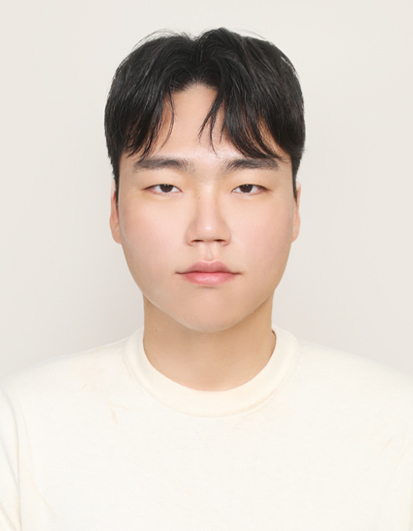
\includegraphics[width=1in,height=1.25in,clip,keepaspectratio]{a1.png}}]{JuneWoo Kang}
is with the Department of Computer Engineering, KwangWoon University, Seoul, South Korea. In 2024, he studied as an exchange student in computer engineering at the University of Nebraska at Kearney (UNK), NE, USA. His major field of study includes computer systems and 3D AI.
He is with MUSTREE and Konkuk University, where he conducts research on enhancing 3D CAD model reconstruction based on Point2CAD pipelines. He was with BlueSolution in Seoul, South Korea, developing user activity tracking systems with C\#, and with AskWhy Valley, teaching elementary and secondary physics. His project experience includes multithreaded and GPU-offloading based performance optimization, web front-end development with TypeScript and Vue, and object-oriented game development in C++.
Mr.\ Kang's technical interests include 3D AI for CAD and geometry processing, backend and full-stack web development, and high-performance computing. His honors include the ROK--US Alliance Scholarship in 2024 and participation in the Kakao Bank Fintech Hackathon in 2025. He is fluent in Korean and proficient in English.
\end{IEEEbiography}

\begin{IEEEbiography}[{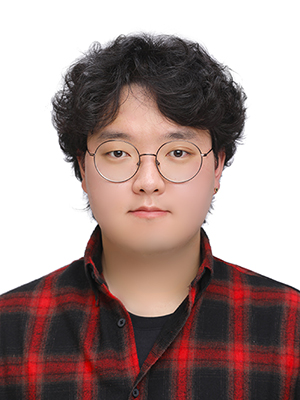
\includegraphics[width=1in,height=1.25in,clip,keepaspectratio]{a2.png}}]{Chaehwan Lee}
was born in Anyang, Gyeonggi-do, South Korea, in 1998. He received the B.S. degree in Mathematics from Kunsan National University, Kunsan, South Korea, in 2024. He is with the Department of Data Science, Konkuk University, Seoul, South Korea.
He is with the Statistical Artificial Intelligence Laboratory at Konkuk University, where he works on reverse engineering and 3D vision–based analysis. His primary research interests include reverse engineering and keypoint-based segmentation. He has participated in projects involving automated reverse engineering, wrinkle measurement using 3D vision, and fine-tuning of LLM. He is currently preparing a patent related to point-cloud–based reverse engineering.
\end{IEEEbiography}

\begin{IEEEbiography}[{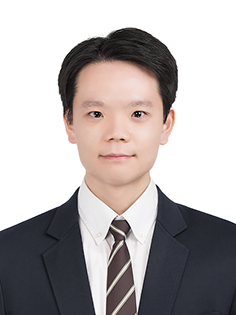
\includegraphics[width=1in,height=1.25in,clip,keepaspectratio]{a3.png}}]{YongHak Lee} received the B.A. degree in statistics in 2020 and the M.S. degree in statistics in 2022, both from Konkuk University in Seoul, South Korea. He is with the Department of Statistics and the Statistical Artificial Intelligence Lab at Konkuk University.
From 2020 to 2021, he was with Deep Visions. Since March 2022, he has been with Mustree. He has authored or co-authored over 12 scholarly articles and has one patent filed with the Korean Intellectual Property Office concerning a method for automatic body circumference measurement. His research interests focus on the application of deep learning and computer vision, specifically in areas such as mobile LiDAR-based 3D body measurement, generative models like Diffusion and Generative Adversarial Networks for data generation, and the implementation of decentralized file storage methods.
\end{IEEEbiography}

\begin{IEEEbiography}[{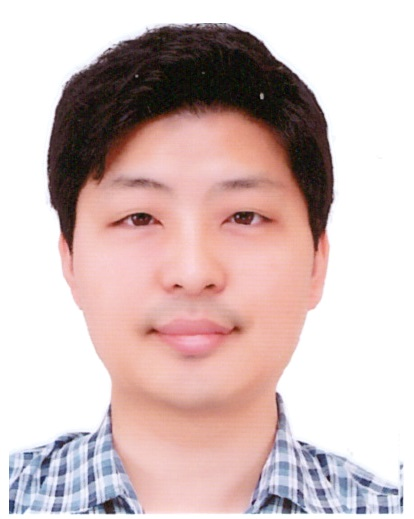
\includegraphics[width=1in,height=1.25in,clip,keepaspectratio]{a4.jpg}}]{Seongmin Yang}
is with the Department of Applied Statistics and the Institute of Applied Statistics, Konkuk University, Seoul, South Korea.
His research interests center on statistical artificial intelligence and computer vision, with a particular focus on object detection and the convergence of statistical modeling with deep learning applications. He initially pursued a background in mathematics education but shifted his focus to statistics, aiming to integrate statistical theory with practical coding capabilities.
Mr. Yang plans to pursue a career in the deep learning industry, applying his expertise in data science and programming.
\end{IEEEbiography}

\EOD
\end{document}